% Options for packages loaded elsewhere
\PassOptionsToPackage{unicode}{hyperref}
\PassOptionsToPackage{hyphens}{url}
%
\documentclass[
]{book}
\usepackage{amsmath,amssymb}
\usepackage{iftex}
\ifPDFTeX
  \usepackage[T1]{fontenc}
  \usepackage[utf8]{inputenc}
  \usepackage{textcomp} % provide euro and other symbols
\else % if luatex or xetex
  \usepackage{unicode-math} % this also loads fontspec
  \defaultfontfeatures{Scale=MatchLowercase}
  \defaultfontfeatures[\rmfamily]{Ligatures=TeX,Scale=1}
\fi
\usepackage{lmodern}
\ifPDFTeX\else
  % xetex/luatex font selection
\fi
% Use upquote if available, for straight quotes in verbatim environments
\IfFileExists{upquote.sty}{\usepackage{upquote}}{}
\IfFileExists{microtype.sty}{% use microtype if available
  \usepackage[]{microtype}
  \UseMicrotypeSet[protrusion]{basicmath} % disable protrusion for tt fonts
}{}
\makeatletter
\@ifundefined{KOMAClassName}{% if non-KOMA class
  \IfFileExists{parskip.sty}{%
    \usepackage{parskip}
  }{% else
    \setlength{\parindent}{0pt}
    \setlength{\parskip}{6pt plus 2pt minus 1pt}}
}{% if KOMA class
  \KOMAoptions{parskip=half}}
\makeatother
\usepackage{xcolor}
\usepackage{longtable,booktabs,array}
\usepackage{calc} % for calculating minipage widths
% Correct order of tables after \paragraph or \subparagraph
\usepackage{etoolbox}
\makeatletter
\patchcmd\longtable{\par}{\if@noskipsec\mbox{}\fi\par}{}{}
\makeatother
% Allow footnotes in longtable head/foot
\IfFileExists{footnotehyper.sty}{\usepackage{footnotehyper}}{\usepackage{footnote}}
\makesavenoteenv{longtable}
\usepackage{graphicx}
\makeatletter
\def\maxwidth{\ifdim\Gin@nat@width>\linewidth\linewidth\else\Gin@nat@width\fi}
\def\maxheight{\ifdim\Gin@nat@height>\textheight\textheight\else\Gin@nat@height\fi}
\makeatother
% Scale images if necessary, so that they will not overflow the page
% margins by default, and it is still possible to overwrite the defaults
% using explicit options in \includegraphics[width, height, ...]{}
\setkeys{Gin}{width=\maxwidth,height=\maxheight,keepaspectratio}
% Set default figure placement to htbp
\makeatletter
\def\fps@figure{htbp}
\makeatother
\ifLuaTeX
  \usepackage{luacolor}
  \usepackage[soul]{lua-ul}
\else
  \usepackage{soul}
\fi
\setlength{\emergencystretch}{3em} % prevent overfull lines
\providecommand{\tightlist}{%
  \setlength{\itemsep}{0pt}\setlength{\parskip}{0pt}}
\setcounter{secnumdepth}{5}
\usepackage{booktabs}
\usepackage{booktabs}
\usepackage{longtable}
\usepackage{array}
\usepackage{multirow}
\usepackage{wrapfig}
\usepackage{float}
\usepackage{colortbl}
\usepackage{pdflscape}
\usepackage{tabu}
\usepackage{threeparttable}
\usepackage{threeparttablex}
\usepackage[normalem]{ulem}
\usepackage{makecell}
\usepackage{xcolor}
\ifLuaTeX
  \usepackage{selnolig}  % disable illegal ligatures
\fi
\usepackage[]{natbib}
\bibliographystyle{plainnat}
\usepackage{bookmark}
\IfFileExists{xurl.sty}{\usepackage{xurl}}{} % add URL line breaks if available
\urlstyle{same}
\hypersetup{
  pdftitle={STC 137 Class Notes},
  pdfauthor={Department of Statistics, University of Pretoria},
  hidelinks,
  pdfcreator={LaTeX via pandoc}}

\title{STC 137 Class Notes}
\author{Department of Statistics, University of Pretoria}
\date{Last Updated: 2025-02-01}

\begin{document}
\maketitle

{
\setcounter{tocdepth}{2}
\tableofcontents
}
\chapter*{Preface}\label{preface}
\addcontentsline{toc}{chapter}{Preface}

In modern society, whether you are reading a magazine, watching TV or scrolling through social media, you encounter statistics. You can't avoid it! Data collection, analysis and communication have become part of day-to-day activities. If you want to be an educated consumer and citizen, you need to understand how statistics are used and also misused in our daily lives. In other words, you need to be \emph{data literate}. The purpose of this book is to give students, in any field of study, a conceptual and practical introduction to the field of statistics. The main focus is on the use of basic statistical techniques for, among others, \emph{collecting data}, \emph{understanding the data} by exploring it, \emph{analyzing the data}, \emph{interpreting the data} and \emph{communicating the data} to facilitate data-driven decision-making. The book is application oriented. The discussion of each technique is followed by application examples. This book is written with the needs of the practitioner in mind. The mathematical prerequisite is matric (Grade 12) level mathematics.

\chapter{An Overview of Data literacy}\label{an-overview-of-data-literacy}

In modern society, we frequently see the following types of statements in the media:

\begin{itemize}
\item
  Momentum Chief Executive, Jeanette Marais, said while 80\% of the {[}withdrawal requests from the two-pot retirement system{]} are from people between 30 and 49 years old, there was concern over requests from the 50-59 age group, which made up 16\% of the total. (Reuters, 27 September 2024)
\item
  Despite the ever presence of sunshine and wind, only 8\% of South Africa's power comes from renewables compared to a global average of 29\%. (IOL.co.za, 11 December 2023)
\item
  BHP Billiton, the Australian-based diversified global miner, says it expects global electricity consumption for data centers to rise from around 2\% of total demand today, to 9\% by 2050, with copper demand in data centers increasing six-fold by then. (Mining.com, 30 September 2024)
\item
  According to StatsSA's latest report, motor trade sales for March 2024 (measured in real terms by constant 2019 prices) decreased by 10.4\% year-on-year, 7\% month-on-month, and 2.9\% quarter-on-quarter. (businesstech.co.za, 16 May 2024)
\item
  Unsurprisingly, a trial found that people with heart disease who were obese or overweight reduced their risk of having a severe cardiovascular event --- including death, stroke or heart attack --- by 20\% when they took semaglutide. (Nature.com, 25 September 2024).
\item
  Released this week, the sixth South African HIV prevalence, incidence, and behaviour Survey (SABSSM VI) found a 7.4\% HIV prevalence rate in the province {[}Western Cape{]} for 2022, down from 8.6\% in 2017. (Mail \& Guardian, 29 September 2024)
\end{itemize}

The numerical facts in the preceding statements -- 80\%, 16\%, 8\%, 29\%, 2\%, 9\%, 10.4\%, 7\%, 2.9\%, 20\%, 7.4\% and 8.6\% - are referred to as \textbf{statistics or statistical information}. This type of information can help us understand the trends in economics, business, health and employment and thus enable us to make more informed decisions. Statistical information is \textbf{data} that has been recorded, classified, organized, related, or interpreted within a framework so that meaning emerges\footnote{\url{https://www150.statcan.gc.ca/n1/edu/power-pouvoir/ch1/definitions/5214853-eng.htm}\href{https://www.media.mit.edu/publications/designing-tools-and-activities-for-data-literacy-learners/}{}}. Thus, an essential skill towards effectively making use of statistical information is data literacy. In this Chapter, we give an overview of data literacy, including key data literacy skills that will be covered more broadly in the coming chapters. Thus, this chapter lays the foundation for the rest of the book.

\section{Introduction}\label{sec1-1}

In modern society, \textbf{data} is everywhere. It is collected when you

\begin{itemize}
\item
  make a purchase online (such as Takealot);
\item
  access a learning management system (such as ClickUP);
\item
  click an advertisement;
\item
  like or comment on someone's social media post;
\item
  stream music or movies online (using platforms such as Spotify and Netflix);
\item
  review your experience with a product or service online (such as our stay at an Airbnb); and
\item
  engage in physical activity and even while you are sleeping! (when you are wearing a fitness tracker such as a Fitbit or Garmin).
\end{itemize}

This implies that data has now become more widely accessible to organizations as well as ordinary individuals. Using this \textbf{data}, organizations (and individuals) can make more data-driven decisions with \textbf{statistics} instead of intuition. This often leads to increased performance and efficiency, especially when compared to less data-driven approaches. However, access to data on its own isn't enough to ensure organizational success. The users of this data, such as the employees in an organization, have to understand and know how to leverage the data and this requires that they have the necessary data literacy skills.

\subsection{Definition}\label{definition}

Bhargava and D'Ignazio (2015), define data literacy as the ability to read, work with, analyze and argue with data\footnote{\url{https://www.media.mit.edu/publications/designing-tools-and-activities-for-data-literacy-learners/}}. Reading the data involves understanding the data and being able to interpret it. Working with data involves creating, acquiring and managing the data. Analyzing the data involves filtering, sorting and aggregation of the data. Arguing with the data means using the data to communicate.

In this book, we adopt an expanded form of the above definition of \emph{data literacy}. We define data literacy as the ability to \ul{manage}, \ul{understand}, \ul{explore}, \ul{analyze}, \ul{interpret} and \ul{communicate} with data in a meaningful way. Data literacy does not require an individual to be an expert but to show an understanding of the basic data fundamentals like data sources, data types, measurement scales, types of analysis, data cleaning, data analysis tools (such as Excel)\footnote{\url{https://online.hbs.edu/blog/post/data-literacy}}, concepts that will be explored in more detail in this book. ~

\subsection{The importance of being data literate in modern society}\label{the-importance-of-being-data-literate-in-modern-society}

In modern society, data plays a pivotal role for the proper functioning of governments, businesses, households and individuals. Being data literate: (1) can lead to timely response to socio-economic or health related issues, (2) it can create sustained economic value, (3) it can assist with making informed decisions, (4) it can improve communication and (5) lead to professional or career advancement. In this section, we briefly discuss the benefits of being data literate for each of these various stakeholders.

\begin{itemize}
\tightlist
\item
  Governments
\end{itemize}

Information from a population census can assist a government official or department to efficiently allocate government resources by, for instance, making sure that there is an equal distribution of services such as health and education.

\begin{itemize}
\tightlist
\item
  Businesses
\end{itemize}

Information from a marketing survey can assist a business to reduce its costs, improve its operational efficiency into operational excellence, improve its competitive advantage and market positioning by, for instance, understanding the trends among its customer base.

\begin{itemize}
\tightlist
\item
  Households
\end{itemize}

Statistical information on the annual government budget can assist households adjust savings strategies based on changes in social welfare; identify job opportunities based on the allocation of public funds to sectors such as construction and make informed decisions through civic participation and democratic engagement. ~

\begin{itemize}
\tightlist
\item
  Individuals
\end{itemize}

Statistical information from a health survey or smart watch can assist an individual to improve their health and well-being; In modern society, misinformation spreads faster and widely often resulting in inaccurate decision-making. A data-literate public is more important today in order to anticipate and prevent the negative consequences of misinformation.

\subsection{Data Literacy Skills}\label{data-literacy-skills}

The essential skills needed in order to be data literate can be divided according to the definition of data literacy as \ul{managing}, \ul{exploring}, \ul{analyzing}, \ul{understanding}, \ul{interpreting} and \ul{communicating} with data. The first three skills are more technical and will be explained in the following chapters. The last three skills are more practical and will be demonstrated in the following section.

\subsection{Data Literacy in Practice}\label{data-literacy-in-practice}

\subsubsection{Being able to interpret or understand and use the information contained in a chart or graph.}\label{being-able-to-interpret-or-understand-and-use-the-information-contained-in-a-chart-or-graph.}

\begin{enumerate}
\def\labelenumi{\arabic{enumi}.}
\item
  The figure below (obtained from the 2022 \emph{South African National HIV Prevalence, Incidence, Behaviour and Communication Survey (SABSSM VI)}\footnote{\url{https://sahivsoc.org/Files/SABSSMVI-SUMMARY-SHEET-2023.pdf}}) shows a map of South Africa (SA) as a \textbf{heatmap}\footnote{A heatmap is a two-dimensional visual representation of data using colors, where the colors all represent different values (\url{https://www.investopedia.com/terms/h/heatmap.asp})}. For each province, the map displays the HIV prevalence, which is the percentage of the population in the province that are HIV positive.

  \begin{figure}
  \centering
  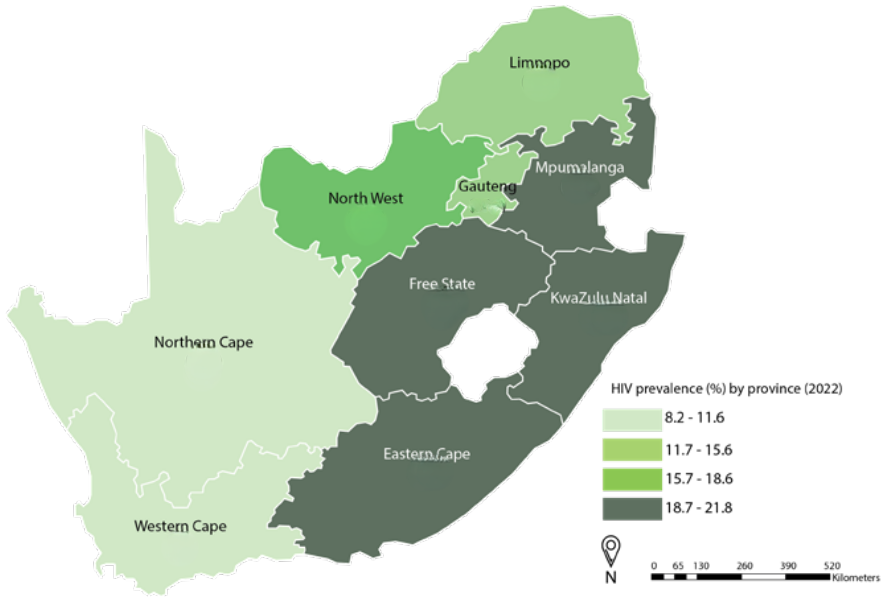
\includegraphics[width=5.20833in,height=\textheight]{images/HIV-Prevalence_2022.png}
  \caption{A heatmap of South Africa showing the HIV prevalence rate in each province in 2022}\label{fig1}
  \end{figure}
\end{enumerate}

From Figure \ref{fig1}, we can see that, in 2022, the Western Cape and Northern Cape had the lowest HIV prevalence (8.2 -- 11.6\%).

\begin{enumerate}
\def\labelenumi{\arabic{enumi}.}
\setcounter{enumi}{1}
\item
  The figure below (Figure \ref{fig2} shows a map (from an article in the September 30, 2024 issue of the \emph{Wall Street Journal}) of the United States of America (USA) as a heatmap. For each state of the USA, the map displays the share of the total power consumed by data centers in 2023. The lighter the section on the map, the less the share of the power consumed by data centers.

  \begin{figure}
  \centering
  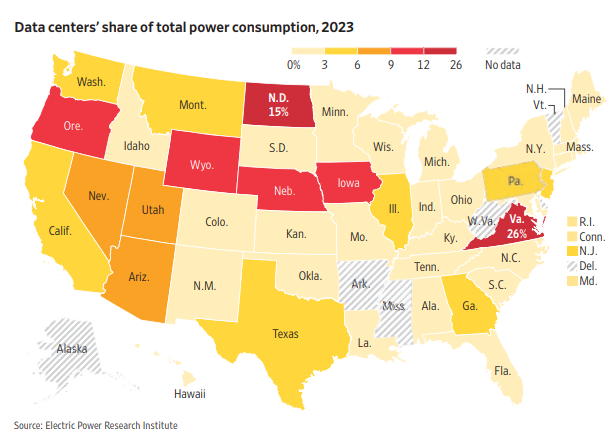
\includegraphics[width=5.20833in,height=\textheight]{images/Data_Centers.png}
  \caption{A heatmap of the United States showing the data centers' share of total power consumption by state in 2023}\label{fig2}
  \end{figure}

  From Figure \ref{fig2}, we can see that in the state of Michigan (Mich.), for instance, data centers consume a small share (0 -- 3\%) of the total power consumed by the state. Whereas, in the state of Virginia (Va.) data centers consume a large share (26\%) of the total power consumed in the state.
\end{enumerate}

\subsubsection{Being able to contextualize a number given in the media:}\label{being-able-to-contextualize-a-number-given-in-the-media}

\begin{enumerate}
\def\labelenumi{\arabic{enumi}.}
\item
  The following is an extract from an article in the Financial Times UK\footnote{\url{https://www.ft.com/content/da407b47-4133-470a-9574-508cee43e107}}

  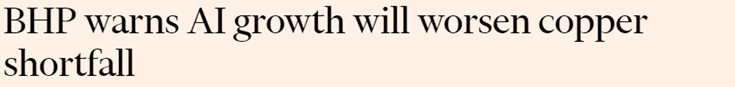
\includegraphics[width=5.20833in,height=\textheight]{images/clipboard-712778398.png}

  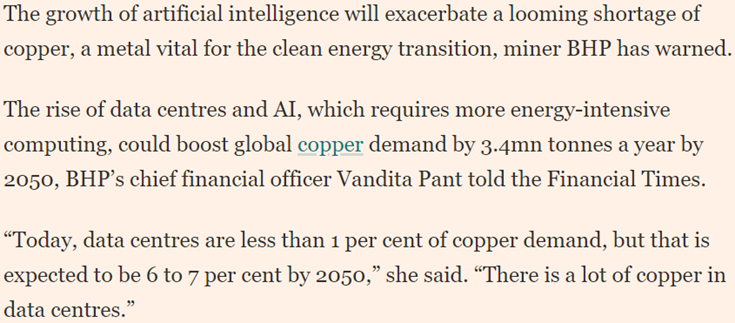
\includegraphics[width=5.20833in,height=\textheight]{images/clipboard-4056060037.png}
\end{enumerate}

The article talks about the growth in future copper demand from data centers as a result of Artificial Intelligence (AI). Data centers are now being used to run AI models and this process is energy intensive. Copper is used in various aspects of a data center\footnote{\url{https://www.visualcapitalist.com/sp/copper-the-critical-mineral-powering-data-centers/}}. The growth in data centers means the growth in copper demand. Today, of all the things copper is used for in the world, data centers account for less than 1\%. This number can grow to 6\% or 7\% by 2050 as a result of an increase of an additional 3.4 million tonnes of global copper demand.

\textbf{Possible implications of the above statistics}: Increased job growth in the copper value chain and construction of data centers; Increased demand for AI and data center expertise; Increased demand for mining engineers with expertise in copper mining.

\subsubsection{Recognising and being able to identify and avoid wrong interpretations of statistical information in the media.}\label{recognising-and-being-able-to-identify-and-avoid-wrong-interpretations-of-statistical-information-in-the-media.}

\begin{enumerate}
\def\labelenumi{\arabic{enumi}.}
\item
  Consider the following extract of an article from the Business Day\footnote{\url{https://www.businesslive.co.za/bd/companies/telecoms-and-technology/2024-09-19-mtn-5g-coverage-up-to-44-of-sa/\#:~:text=Mobile\%20operator\%20concludes\%20deployment\%20scope,sites\%20fitted\%20with\%20the\%20technology&text=MTN\%20has\%20grown\%20its\%205G,than\%2098\%25\%20of\%20the\%20country}}

  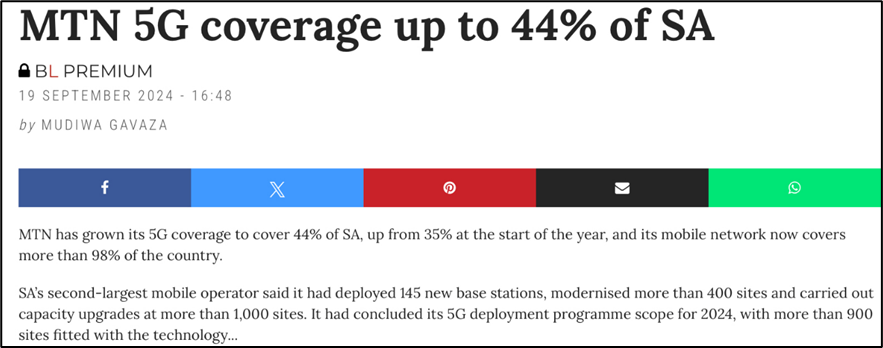
\includegraphics[width=5.20833in,height=\textheight]{images/clipboard-338848850.png}

  How can we interpret the statistical information of 44\% and what are its implications?

  \textbf{What it means}:

  44\% of the total land area in South Africa has access to MTN's 5G network signal.

  \textbf{What it \ul{doesn't} mean}:

  44\% of South Africans use MTN's 5G mobile network.
\end{enumerate}

\begin{enumerate}
\def\labelenumi{\arabic{enumi}.}
\setcounter{enumi}{1}
\item
  The United States' (US) Center for Disease Control (CDC) reported that 99\% of the monkeypox cases in the US occurred in men.

  \textbf{This means that:}

  Of all the reported monkeypox cases in the US, 99\% of them were men.

  \textbf{It doesn't mean that:}

  All the monkeypox cases in the US are men. Thus, falsely, implying that men are more likely to get monkeypox (99\% chance!).
\end{enumerate}

\subsection{Exercises to Section 1.1}\label{exercises-to-section-1.1}

\textbf{Question 1}

What is data literacy?

\textbf{Question 2}

In each of the following scenarios, identify the statistical information:

\begin{enumerate}
\def\labelenumi{\alph{enumi}.}
\item
  A recent poll showed that 30\% of South African wealth is held by the top 1\% of the wealthy individuals in the country.
\item
  An environmental survey revealed that females were more environmentally conscious than males.
\item
  A health study showed that people with nausea are more likely to have headaches.
\item
  In a retirement planning survey, the majority of people who responded were under the age of 35.
\end{enumerate}

\textbf{Question 3}

Answer the following as True or False.

\begin{enumerate}
\def\labelenumi{\alph{enumi}.}
\item
  Data literacy is only useful to data analysts, statisticians and data scientists.
\item
  It is not necessary to have an advanced knowledge in Statistics in order to be data literate.
\item
  One of the skills of data literacy is the ability to argue with data.
\item
  Data literacy can improve my communication skills.
\end{enumerate}

\textbf{Question 4}

Answer the following questions based on Figure \ref{fig1}.

\begin{enumerate}
\def\labelenumi{\alph{enumi}.}
\item
  What is the HIV prevalence rate for the North West province?
\item
  Which of the nine provinces have the largest HIV prevalence?
\item
  Which one of the following provinces has the highest HIV prevalence?

  \begin{enumerate}
  \def\labelenumii{\roman{enumii}.}
  \item
    North West
  \item
    Limpopo
  \item
    Gauteng
  \end{enumerate}
\item
  How many coastal provinces have the largest HIV prevalence (18.7 -- 21.8\%) and how many inland provinces have the largest HIV prevalence?
\end{enumerate}

\textbf{Question 5}

Answer the following questions based on Figure \ref{fig2}.

\begin{enumerate}
\def\labelenumi{\alph{enumi}.}
\item
  What share of the total power consumption in the state of Washington (Wash.) is used by data centers?
\item
  Which of the following states has the largest share of its total power consumed by data centers?

  \begin{enumerate}
  \def\labelenumii{\roman{enumii}.}
  \item
    Texas
  \item
    Nebraska (Neb.)
  \end{enumerate}
\end{enumerate}

\textbf{Question 6}

Consider the following figures (from the May 6, 2024 issue of \emph{Barrons' Magazine}) which summarizes the responses by professional investment managers on their outlook on: (\textbf{\emph{left figure}}) public USA companies (Bullish means they have a positive outlook, bearish means they have a negative outlook and neutral means they are neither positive nor negative.) and (\textbf{\emph{right figure}}) which global public equity market they think will perform the best.

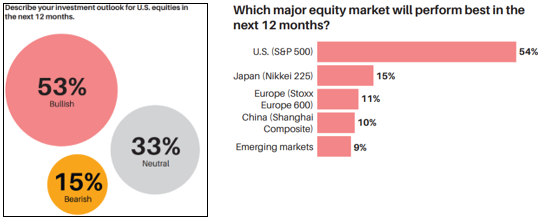
\includegraphics{images/Section 1 - 1.png}

\begin{enumerate}
\def\labelenumi{\alph{enumi}.}
\item
  What can you say about the outlook of the majority of managers on USA public companies?
\item
  Which global public equity market is the least favored?
\item
  Something is wrong with these figures, can you identify it?
\end{enumerate}

\textbf{Question 7}

For each of the following statements, state whether or not the interpretation of the statement is accurate. If not, motivate your answer.

\begin{enumerate}
\def\labelenumi{\alph{enumi}.}
\item
  Of all the people born in Gauteng, 25\% of them speak Sotho. Therefore, for anyone who speaks Sotho, there is a 25\% chance/probability that they were born in Gauteng.
\item
  The potato yield in the Limpopo province was found to be positively correlated with the coal production in the Mpumalanga province. Therefore, high potato yields lead to increases in coal production. ~
\item
  About 75\% of the South African population has access to the internet. In other words, this implies that 3 in 4 South African citizens have some form of access to the internet.
\end{enumerate}

\newpage

\section{Data}\label{data}

\subsection{What is data?}\label{what-is-data}

Data are the raw facts and figures, about objects or events, that are collected, analyzed and summarized for presentation and interpretation in order to make informed decisions. Data typically arises as a result of a \textbf{study}. For instance, suppose the South African Reserve Bank (SARB) wants to forecast inflation in the next 12 months (the study). They will collect data about the inflation rate in the previous years and other factors influencing inflation. All the data collected by the SARB is referred to as a \textbf{data set}.

Table 1 gives a data set containing information about the 9 provinces of South Africa. The data was obtained from the 2022 South African census. The South African census is conducted every 10 years. A census provides information on the demographic, socioeconomic and geographic characteristics of the entire population, as well as household characteristics.

\begin{figure}
\centering
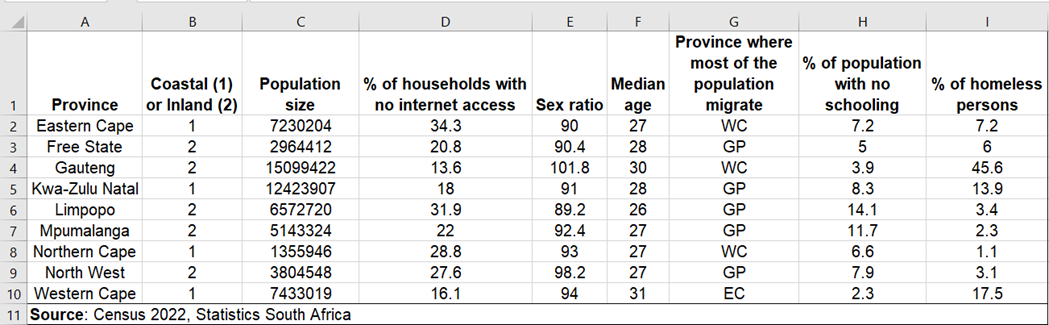
\includegraphics{images/clipboard-533064056.png}
\caption{Table 1: Data set on information about the 9 provinces of South Africa}
\end{figure}

\subsection{Properties of a data set}\label{properties-of-a-data-set}

Any data set has three essential properties, namely

\subsubsection{Elements}\label{elements}

These are the entities or objects on which the data are collected. Each of the nine provinces in Table 1 are the elements of the data.

\subsubsection{Variables}\label{variables}

These are the characteristics of interest about the elements. The data set in Table 1 has eight variables:

\textbf{Coastal or Inland}: The province's area of location in South Africa; It can be either coastal or inland.

\textbf{Population size}: The number of people in a province.

\textbf{\% of households with no internet access}: The number of households that have no access to the internet in a province as a percentage of the total population in a province.

\textbf{Sex ratio}: The number of males for every 100 females in a province. A value above 100 indicates that there are more males than females.

\textbf{Median age}

\textbf{Province where most of the population migrate}: A province in South Africa where most of the population in another province migrate to.

\textbf{\% of population with no schooling}: The number of persons in a province with no formal schooling as a percentage of the total number of persons in the province.

\textbf{\% of homeless persons}: The number of homeless persons in a province as a percentage of the total number of homeless persons in South Africa.

\subsubsection{Observations}\label{observations}

These are the sets of measurements obtained from each element. From Table 1, the first element (Eastern Cape) has the following measurements:

\begin{longtable}[]{@{}llllllll@{}}
\toprule\noalign{}
\endhead
\bottomrule\noalign{}
\endlastfoot
1 & 7230204 & 34.3 & 90 & 27 & WC & 7.2 & 7.2 \\
\end{longtable}

The second element (Free State) has the following measurements:

\begin{longtable}[]{@{}llllllll@{}}
\toprule\noalign{}
\endhead
\bottomrule\noalign{}
\endlastfoot
2 & 2964412 & 20.8 & 90.4 & 28 & GP & 5 & 6 \\
\end{longtable}

and so on. The data set with 9 elements has 9 observations.

\subsection{Observational and experimental data}\label{observational-and-experimental-data}

Data can come from an observational study or an experimental study. \textbf{Observational data} are records of what is actually taking place in a particular situation. The data in Table 1 are an example of observational data. As another example of observational data, a bank might observe client visits at one of their branches to collect data on variables such as the length of time a typical client spends at the branch, the number of clients visiting the branch on a given day (e.g.~Monday or last day of the month), the age of the clients and so on. Statistical analysis of this data may, for instance, help bank management decide whether or not to close the branch in order to reduce operational costs.

\textbf{Experimental data} is data that is obtained under controlled conditions. It is typically used to test a hypothetical statement. For instance, suppose a pharmaceutical company would like to test whether a new drug they developed is effective for weight loss. To obtain the data, researchers select a sample of individuals. The individuals are instructed to follow the same diet. One group (treatment group) of individuals is given a dose of the new drug and another group (control group) is not given the new drug. After two months, we collect data on the weight of individuals in each group and compare it with the weight data collected before the experiment. Statistical analysis of the data can help determine whether the average weight loss of the treatment group is significantly greater than that of the control group.~

\subsection{Cross-sectional and time-series data}\label{cross-sectional-and-time-series-data}

For appropriate analysis, interpretation and communication with the collected data, a distinction must be made between \textbf{cross-sectional data} and \textbf{time series data}. Cross-sectional data are data collected at the same point in time about two or more elements. The data in Table 1 are cross-sectional because they describe eight variables about the nine provinces (elements) at the same point in time (2022). Time series data are data collected over several time periods. For instance, the figure below shows the estimated Life Expectancy at birth in South Africa for the period 2002 to 2024. Time series plots, such as the figure below, are very useful in understanding what happened in the past, identifying whether there are any trends over time and, often, forecast future values of the time series.

A time series plot is typically easy to understand and interpret. For example, from the figure, we can see that life expectancy at birth declined between 2002 and 2006. Incidentally, this was a period of increasing HIV prevalence and lack of awareness and information about prevention measures. However, due to increased awareness of HIV, expansion programmes to prevent mother-to-child transmission coupled with access to ARVs, life expectancy at birth increased from 2006 before declining in 2020 due to COVID-19.~

\begin{figure}
\centering
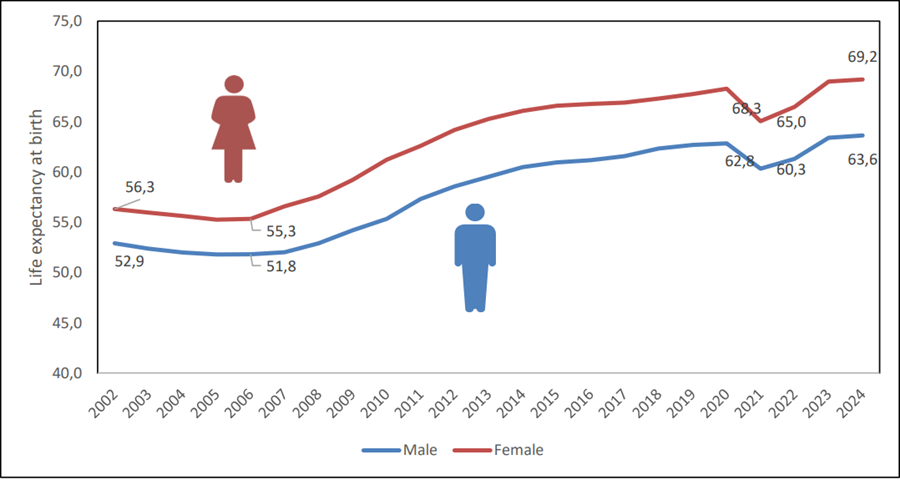
\includegraphics[width=5.20833in,height=\textheight]{images/clipboard-2840066963.png}
\caption{Figure: Life expectancy at birth in South Africa over time 2002 -- 2024}
\end{figure}

\subsection{Population and sample}\label{population-and-sample}

Typically, the elements in a study consist of a large number of objects or events. For instance, suppose an accounting firm, such as KPMG, wants to determine whether the amount of accounts receivable reflected on a client's financial statement fairly represents the actual amount of accounts receivable. Usually large industrial or manufacturing businesses, such as Bidvest Group, will have a large number of accounts receivables which will make reviewing and validating every account too costly and time-consuming. As a common practice, the audit staff selects a subset of all the accounts. This subset of accounts is known as a \textbf{sample} and all of the accounts receivable are known as a \textbf{population}. The process of collecting the data is called \textbf{sampling}.

Note that, although the elements of the data in Table 1 are the provinces, the data itself was collected from individuals from the population of South Africa. Therefore, the elements in a census survey or study are a population.

\subsection{Exercises to Section 1.2}\label{exercises-to-section-1.2}

\textbf{Question 1}

What is a data set?

\textbf{Question 2}

Name the properties of a data set.

\textbf{Question 3}

In 2023, FNB commissioned a retirement survey to find out how prepared South African consumers were for retirement. Is the data obtained from the survey respondents experimental or observational?

\textbf{Question 4}

Suppose a study is conducted to find out whether vaping (or e-cigarette smoking) is less harmful compared to tobacco smoking. Is the data obtained from the study experimental or observational?

\textbf{Question 5}

The figure below gives a bar chart showing the annual revenue of Shoprite over a ten-year period from 2014 to 2023 (The data were obtained from the annual financial statements of Shoprite\footnote{\url{https://www.shopriteholdings.co.za/shareholders-investors/financial-results-archive.html?p=1}} and the graph was plotted using Excel).

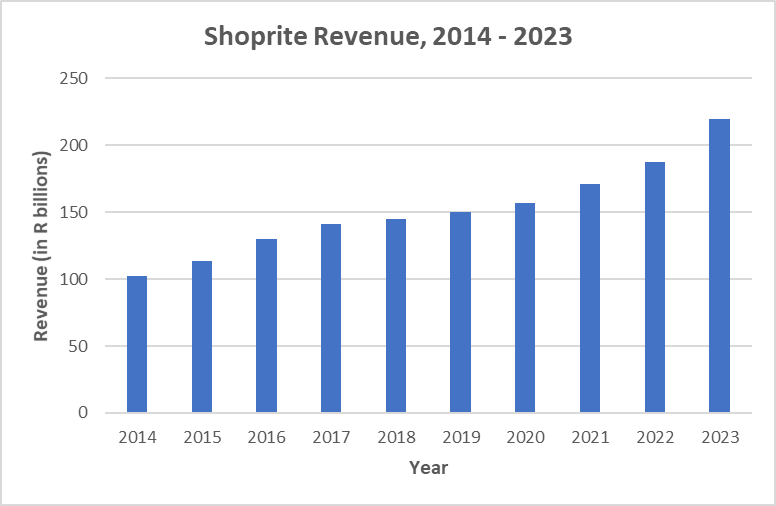
\includegraphics[width=5.20833in,height=\textheight]{images/clipboard-3088691256.png}

a. What is the variable of interest?

b. Are the data cross-sectional or time-series?

c. What can you say about the trend in Shoprite's revenue overtime?

\textbf{Question 6}

The figure below shows the quarterly FNB/BER Consumer Confidence Index for the period 2014, 1\textsuperscript{st} quarter, to 2024, 2\textsuperscript{nd} quarter\footnote{\url{https://www.fnb.co.za/blog/investments/articles/EconomicsWeekly-20240913/?blog=investments&category=Economics&articleName=EconomicsWeekly-20240913}}. The index measures confidence among South African consumers based on their outlook on the economy and their household financial position. A higher value indicates high confidence\footnote{\url{https://www.ber.ac.za/Documents/Index/FNBBER-Consumer-Confidence-Index}}.

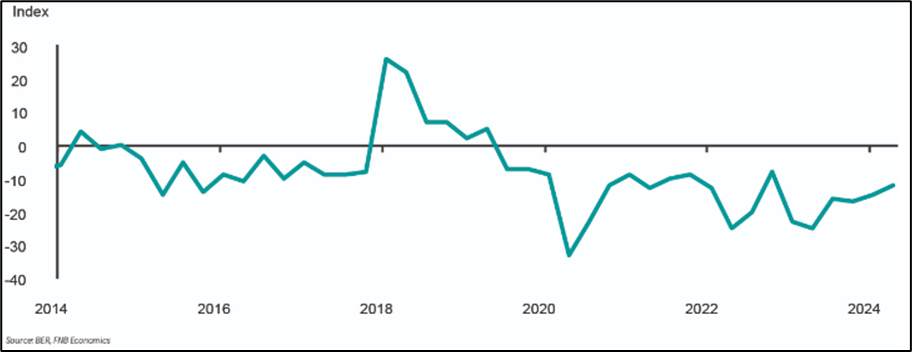
\includegraphics[width=4.16667in,height=\textheight]{images/clipboard-2186963206.png}

\begin{enumerate}
\def\labelenumi{\alph{enumi}.}
\item
  Are the data cross-sectional or time-series?
\item
  Comment on the confidence of the South African consumer over time.
\end{enumerate}

\hfill\break
\textbf{Question 7}

The South African Bureau of Economic Research collects data from South African adults living in predominantly urban areas to measure consumer confidence in South Africa. Survey respondents are asked about

\begin{itemize}
\item
  their expectation about the performance of the economy;
\item
  their expectation about the financial position of households;
\item
  their rating of the present time to buy durable goods (e.g.~electronic appliances).

  \begin{enumerate}
  \def\labelenumi{\alph{enumi}.}
  \item
    What is the population being studied?
  \item
    Is surveying mostly people in the urban areas a good way to get a good picture of consumer confidence in a country like South Africa?
  \end{enumerate}
\end{itemize}

\textbf{Question 8}

The 2024 Annual FNB Retirement survey collected data from a sample of 1072 South African consumers to, amongst other things, uncover their preparedness for retirement. Almost half of the respondents indicated that they do not have a retirement plan in place and 20\% of the respondents indicated an annual income of more than R 850 000.

\begin{enumerate}
\def\labelenumi{\alph{enumi}.}
\item
  What is the population of interest in this survey?
\item
  Is the data collected from the survey observational or experimental?
\item
  Does this survey involve cross-sectional data or time-series data?
\item
  Describe any useful insights for FNB that can be obtained from the collected data.
\end{enumerate}

\newpage

\section{Data Management - Foundations and Concepts}\label{sec1-3}

Data management is the practice of collecting, organizing, preparing, protecting and storing data so that it can be used efficiently, securely and cost-effectively in the decision-making process. In modern society, data of different types is generated in large volumes from a variety of sources at an unprecedented speed, thus a robust data management solution is important to extract meaningful and enduring value from the data. Over and above the latter, data management is important to facilitate ease of data migration and transformation and also for regulatory compliance.

\subsection{Data management process}\label{data-management-process}

The data management process is made up of the following components:

\begin{itemize}
\item
  \textbf{Data collection} is the process of gathering the necessary data from the various data sources about the variables of interest for a particular study. This process typically involves a process referred to as sampling (see Chapter \ref{ch4}).
\item
  \textbf{Data organization} involves integrating different types of data, such as structured and unstructured data (see Chapter \ref{ch2}). This process is also referred to as data warehousing.
\item
  \textbf{Data preparation} involves cleaning and transforming raw data into a form that is suitable for further processing and analysis. This process is important for identifying and removing errors and duplicates in the data and also filling in missing data. This increases the accuracy and quality of the data. Data preparation is also known as data wrangling (see Chapter \ref{ch3}).
\item
  \textbf{Data governance} involves, amongst others, the processes and practices used to ensure data protection, security and privacy. \textbf{Data protection} includes safeguarding the data and restoring important information in the event of say, a data breach. \textbf{Data security} refers to safeguarding the data against theft, corruption and unauthorized access. \textbf{Data privacy} refers to safeguarding the collection, use and disclosure of personal and sensitive data to comply with policy and regulation such as the Protection of Personal Information Act (POPIA) of South Africa.
\item
  \textbf{Data storage} involves the retention of the data for future access. In modern society, data is usually stored in a digital format using an SQL database or a spreadsheet. The data files are kept on a personal computer or, in the case of large volumes of data (so-called Big Data), on servers, also known as cloud storage.
\end{itemize}

\subsection{The benefits of data management in modern society}\label{the-benefits-of-data-management-in-modern-society}

At its core, the benefits of an effective data management system include:

\begin{itemize}
\item
  \textbf{Availability and visibility} -- effective data management increases the visibility of the data by making it easily accessible. This in turn leads to high frequency data-driven decision-making.
\item
  \textbf{Reliability} -- a good data management system leads to accurate decision-making by making sure that the data is reliable and up to date. ~~~
\item
  \textbf{Security} -- a good data management system protects the data against loss and ransom-ware type data breaches. Moreover, it ensures that the data are used within the bounds of policy and regulation in an ethical manner.
\item
  \textbf{Scalability} -- a good data management system can allow repeatable data queries that build upon each other and thus keep the data up to date. Moreover, this mitigates inconsistencies and duplications of queries.
\end{itemize}

\subsection{The challenges of data management in modern society}\label{the-challenges-of-data-management-in-modern-society}

As is the case with any useful strategy, there are challenges towards effective data management. These includes, among others,

\begin{itemize}
\item
  The size (or volume) of the data collected

  As mentioned in Section \ref{sec1-1}, data is everywhere. Given the size of the data generated today, traditional storage devices with storage capacity of up to gigabytes (GB) are no longer enough. We need data storage infrastructure with capacity up to terabytes (TB: \textasciitilde1000 GB) and petabytes (PB: \textasciitilde1000 TB).
\item
  The speed (or velocity) at which the data is generated

  Since data is collected at every second of every minute, we need sophisticated infrastructure to quickly effect the changes and keep the data up-to-date for future analysis.
\item
  The variety (or integration) of the data

  Data can come from multiple sources (e.g.~social media and drone), types (e.g.~structured and unstructured data) and formats (e.g.~text and videos). This requires sophisticated infrastructure for data integration.
\item
  The veracity (or quality) of the data

  Given the variety of the data coupled with the speed at which data is generated, it raises a concern over the accuracy and consistency of the information. This can lead to duplication and errors in the data.
\item
  Changing rules and regulations

  The storage and use of data must comply with personal data protection rules and regulations while preventing cyber-attacks.
\item
  Data security and privacy

  Protecting sensitive data while ensuring compliance with data regulations and preventing unauthorized access while ensuring data accessibility for rapid data-driven decision-making.
\end{itemize}

\subsection{Strategies for data management}\label{strategies-for-data-management}

The following strategies can address some of the major data management challenges that organizations face in modern society:

\begin{itemize}
\item
  Data security and access control

  Develop a multi-layered data security system that has a robust role-based access control and data encryption system with clear audit trails.
\item
  Data integration improvement

  Develop a robust ETL (Extract, Transform and Load) process to extract data from various sources and transform it into a standardized format which can be loaded into a central storage system.
\item
  Data quality improvement

  Develop data validation rules, data profiling processes (such as analyzing and assessing the data to gain insights into its consistency and completeness) and error detection and correction procedures.
\item
  Data storage and cost optimization

  Implement a tiered data storage solution with a balance between on-premises and cloud in order to optimize the use of storage and reduce data processing costs.
\item
  Data speed optimization

  Develop a data indexing system for quick data access. Implement caching\footnote{Caching is to temporarily store data so that future requests for the data can be accessed faster.} strategies to reduce the number of database queries and improve the response times.
\end{itemize}

\subsection{Exercises to Section 1.3}\label{exercises-to-section-1.3}

\textbf{Question 1}

What is data management?

\textbf{Question 2}

The National Health Laboratory Services experienced a data breach which led to delays in processing laboratory tests across public health facilities in Gauteng.

\begin{enumerate}
\def\labelenumi{\alph{enumi}.}
\item
  Which one of the following actions should be taken to ensure that the data can be quickly recovered should this happen in the future?

  \begin{enumerate}
  \def\labelenumii{\roman{enumii}.}
  \item
    Improve data privacy
  \item
    Improve data protection
  \item
    Improve data storage
  \item
    Improve data security
  \item
    Optimize data integration
  \end{enumerate}
\item
  Which one of the following actions should be taken to ensure that patient's personal information is not compromised should this happen in the future?
\item
  Improve data privacy
\end{enumerate}

\begin{enumerate}
\def\labelenumi{\roman{enumi}.}
\setcounter{enumi}{1}
\item
  Improve data protection
\item
  Improve data security
\item
  Improve data storage
\item
  Optimize data integration
\end{enumerate}

\textbf{Question 3}

For each of the following scenarios, what do you think is likely to become a challenge in data management? Motivate your answer.

a. TymeBank, a digital bank, is reportedly on-boarding up to 5000 customers every day (that is, about 150000 customers every month).

b. A startup bank insurance (bancassurance) company collects its client's data from cameras in their homes, smart watches and banking transactions.

c. A major South African bank and a life insurance company decided to merge their businesses. When it came to combining their client's data, they failed to notice duplicates because of different data formats.

d. The University of Pretoria and University of Johannesburg are collaborating on a clinical trial for a new cancer drug. Researchers on both sides tend to store sensitive data on their personal computers and they use different names for the data files.

e. Researchers at the United Nations Convention on Climate Change are conducting an environmental monitoring study. Their sensors are collecting data in different formats, they have no backup system for their data and there is no access control on the data.

\newpage

\section{Data Ethics}\label{sec1-4}

Data ethics refers to the principles or practices that seek to preserve the trust of the owners of data, from how the data is collected to how it is stored and used. In essence, data ethics concerns the measures put in place to ensure that the data are handled appropriately throughout the data management process. This is an important issue in modern society given value and ubiquitous nature of data.

\subsection{The importance of data ethics}\label{the-importance-of-data-ethics}

The following real-world examples are meant to demonstrate the consequences of unethical data management thus highlighting the importance of embedding ethical data management principles:

\begin{itemize}
\item
  In June 2018, Liberty Holdings, Africa's largest life insurance company, suffered a major data breach in which hackers access confidential client information. This raised the concern of how organizations protect and store their client's data.
\item
  In September 2021, the South Africa Department of Justice experienced a ransomware attack in which the department's IT systems were compromised affecting all electronic services such as bail services, email and the departmental website. This attack raised concerns over whether government systems are adequately secured, given that they manage sensitive citizen data.
\item
  In October 2017, the Master Deeds experienced a massive data leak that exposed approximately 60 million South African citizens' personally identifiable information (PII) such as ID numbers, contact details and addresses. The data was later found on a public and unsecured server. This incident raised concerned over people's right to privacy. Furthermore, this revealed a poor or no strategy for data governance.
\end{itemize}

These examples are a small snapshot of the poor management of data and its consequences for the owners of the data. Thus, ethical data management principles are important in order to:

\begin{itemize}
\item
  protect customer and, in general, human rights.
\item
  protect customer or client loyalty to your business and society as a whole.
\item
  ensure regulatory compliance and avoid penalty costs.
\item
  reduce and, at best, prevent data breaches.
\end{itemize}

Regardless of who you are, the significance of data ethics is apparent. Although data is a powerful asset that can be used to drive innovation and improve lives, without ethical safeguards, it can also be misused and thus leading to harm.

Understanding data ethics enables us to better navigate how our information is used, ensuring that we can protect ourselves while still engaging in a data-drive society.

\subsection{Data ethics principles}\label{data-ethics-principles}

The following are some of the fundamental principles that can guide ethical data management:

\begin{itemize}
\item
  \textbf{Ownership:} Each individual's personal information is owned by themselves. It is therefore unlawful and unethical to collect information about an individual without their \ul{consent}. It can in fact be considered stealing. \ul{Consent} can be obtained from individuals through written agreements, agreeing toterms and conditions and accepting cookies on websites.
\item
  \textbf{Transparency:} The individual whose data is collected has the right to know how it will be stored and used. It is therefore important for a company to publish a data policy documentation that will explain to the individuals how the data will be stored, why it is collected and how will it be used.
\item
  \textbf{Privacy:} It is important that the company collecting and using personal information of individuals ensure that the information is kept private. Just because the individual gave the company consent to collect personal information, does not mean they want the information to be made public. Such information includes names, surnames, home address, contact information etc. The company should ensure that the data is securely stored so that it cannot end up in the wrong hands through hacking. When working with the data it can also be anonymised by removing the personal information so that an individual cannot be identified through the data.
\item
  \textbf{Intention:} Before collecting data, one should clearly state why they need the data, what they will gain from using it and what possible changes, if any, will they make after making use of the data. If your intentions are to use the data to cause harm or for any other bad reason, it is unethical. Therefore, when collecting data it is important to do so with good intentions. Also, do not collect any data that is not necessary for the end goal.
\item
  \textbf{Accountability:} The company collecting the data must take responsibility for the data collected including protecting it from data breaches and misuse. This important for maintaining trust between the company and its clients.
\item
  \textbf{Bias:} The data as well as the algorithms used for the analysis should not have any inherent biases that will skew the results. Such biases can include amongst others racial, gender and socioeconomic biases.
\end{itemize}

\subsection{Exercises to Section 1.4}\label{exercises-to-section-1.4}

\textbf{Question 1}

Which of the following is NOT a key principle of ethical data use?

a. Privacy

b. Bias

c. Profit maximization

d. Transparency

\textbf{Question 2}

What does ``informed consent'' mean in the context of data collection?

a. Data subjects must be informed about the specific use of their data and must voluntarily agree to it.

b. Data subjects must be forced to share data if it benefits society.

c. Data subjects should be informed only after data collection has taken place.

d. Data can be collected without consent if it is anonymised.

\textbf{Question 3}

What is ``data minimization'' in data ethics?

a. Limiting data collection to the minimum amount needed to achieve the stated purpose.

b. Deleting data after analysis to reduce storage costs.

c. Sharing data only with third parties who minimize its use.

d. Using smaller datasets for faster processing.

\textbf{Question 4}

Explain the concept of ``bias'' in data and why it can lead to unethical outcomes.

\textbf{Question 5}

What are the potential ethical concerns with using personal data collected for one purpose (e.g., marketing) for a different purpose (e.g., medical research)?

\newpage

\section{Data Exploration -- Foundations and Concepts}\label{sec1-5}

Data exploration is an important first step in the data analysis process. It involves uncovering the characteristics, patterns and hidden insights in the observed data set in an effort to gain a deeper understanding of the data. This step is usually referred to as exploratory data analysis (EDA). During EDA, statistical techniques are used to look for similarities, patterns, anomalies and also identify relationships between the different variables in the raw data. This step is also important for investigating the quality of the data by identifying missing values, duplicate data entries and\textbackslash or inconsistencies in the data. Data exploration can be seen as part of, or as following, the data preparation step in the data management process.

\subsection{Approaches to exploratory data analysis}\label{approaches-to-exploratory-data-analysis}

\begin{itemize}
\item
  \textbf{Descriptive statistics} are the main numerical features of the data such as the central tendency of the data (using the mean or median) and the spread of the data (using the variance or standard deviation). For instance, suppose you are a quantitative analyst working for a bank and you have a spreadsheet of the loan amounts given out during the current financial period. A descriptive analysis, such as calculating the mean and standard deviation of the loan amount, can give you the average loan amount and the dispersion in the loan amounts, respectively. As another example, suppose we want to understand the relationship between wind speed and air temperature, we can calculate the covariance to identify whether there is a relationship between these variables, and if so, is it positive or negative. Moreover, we can calculate the correlation coefficient to quantify the strength of the relationship.
\item
  \textbf{Tabular and graphical statistics} are summaries and interpretations of the data using graphs and tables. This is useful for identifying trends and relationships between numerical variables (using scatter plots) and categorical variables (using cross-tabulations), distributional patterns (using histograms, frequency distributions and the ogive) and outliers (using a box-and-whisker plot). For instance, the figure below shows a box and whisker plot of a sample of data. It can be seen from the figure that the data point marked ``Outlier'' might be unusual in relation to the rest of the data.
\end{itemize}

\begin{figure}

{\centering 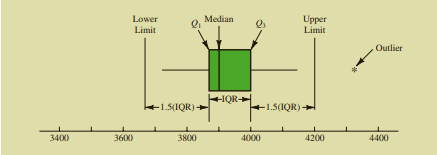
\includegraphics[width=0.8\linewidth]{Figures-Chapter1/Outlier} 

}

\caption{A box-and-whisker plot showing an outlier}\label{fig:unnamed-chunk-3}
\end{figure}

\begin{itemize}
\tightlist
\item
  \textbf{Inferential statistics} uses sampled data to draw conclusions about the population. This includes testing various hypotheses statements you may have about the population where the data was obtained such as whether certain variables follow a specific distribution or whether the observed relationship between two or more variables, from a graph, is significant. For instance, suppose that you are a quantitative analyst for a bank and you want to test the hypothesis that the average loan amount for male clients is large than that of female clients. This type of test can be easily performed using the Data Analysis tool in Microsoft Excel.
\end{itemize}

\subsection{Advantages and disadvantages of data exploration}\label{advantages-and-disadvantages-of-data-exploration}

Data exploration has several benefits, including:

\begin{itemize}
\item
  Offering a comprehensive understanding of the data set before conducting the actual analysis.
\item
  Enhancing the quality of the data.
\item
  Highlighting important features and potential issues
\item
  Providing insight into appropriate analysis techniques~
\item
  Guiding future research questions and directions
\end{itemize}

Limitations of data exploration may include:

\begin{itemize}
\item
  Difficulty visualizing the high-dimensional data
\item
  May become complex for complicated data structures
\item
  It can be time consuming and subjective.
\item
  Misrepresenting data by choosing the wrong summary indicators
\end{itemize}

\subsection{Stages in the exploratory data analysis process}\label{stages-in-the-exploratory-data-analysis-process}

The data exploration process involves a series of stages or steps which are aimed at obtaining a comprehensive understanding of the data and the implications thereafter. This includes

\begin{enumerate}
\def\labelenumi{\arabic{enumi}.}
\item
  Understand the problem understudy

  A crucial first step in the EDA process is to clearly state the problem that led to the collection of the data. This will help in various ways, such as formulating relevant questions, choosing the appropriate analytical tools and identifying inconsistencies or anomalies in the data.
\item
  Examine the structure of the data

  Once you have a clear understanding of the problem, the next step is to familiarise yourself with the data by examining its structure which includes the size of the data, the number of variables and their data types. Check for inconsistencies and anomalies in the data and also missing values or data entries.
\item
  Handle the inconsistencies, anomalies and missing values

  The next crucial step is to have a strategy to handle any inconsistencies, anomalies and\textbackslash or missing data entries identified in the second step.
\item
  Examine the statistical aspects of the data

  After addressing the issues identified in the second step, the next step involves the examination of the distribution, central tendency and variability of all the numerical variables. Moreover, various assumptions about the data can be tested. Among other things, this exercise will assist in identifying variables that deviate from expected patterns and may need further processing.
\item
  Transform the data for analysis

  The next step is to prepare the data to be ready for data analysis. Based on your insights from the previous step, you may have to apply certain transformations to the data to make them conform to expectations. This involves, among others, standardizing or normalizing numerical variables, taking the log or square root to correct for skewness in numerical variables and dummy coding categorical variables.
\item
  Visualize the data

  After transforming the data, you can now visualize it using tables and graphs such as frequency distributions and histograms. Data visualization is covered in some detail in Section \ref{sec1-6}.
\item
  Communicate the findings and use them for further data analysis.
\end{enumerate}

\subsection{Exercises to Section 1.5}\label{exercises-to-section-1.5}

\textbf{Question 1}

What is data exploration?

\textbf{Question 2}

For each of the following scenarios, identify the approach used for data exploration:

a. A research team analysed the health data of City of Tshwane residents. They found that 12\% of the residents have at least one non-communicable disease.

b. An environmental scientist analysed data on monthly carbon dioxide (CO\textsubscript{2}) emissions and the monthly number of people hospitalized for respiratory issues in Pretoria. A scatter plot showed that there is a positive relationship between these two variables.

c. A fitness instructor analysed data on the exercise patterns of people in the district of the Cape Winelands in the Western Cape. She plotted the data on a histogram and found a bimodal distribution of exercise habits, suggesting that there are two distinct behavioural groups.

d. A marine biologist analysed data collected over 10 years by sensors from the bottom of the Indian ocean. She found that the average temperature was 24 degrees Celsius.

e.A hospital administrator at Hatfield General hospital claims that less than 10\% of the daily hospital admissions are for serious injuries. In an analysis of hospital data, he was able to confirm his claim.

\newpage

\section{Data visualization -- Foundations and Concepts}\label{sec1-6}

According to the \href{https://hbr.org/2016/06/visualizations-that-really-work}{Harvard Business Review}, data visualization is a must-have data literacy skill for junior and even senior management. This is because it provides the only way for them to make sense of the work they do. As the world becomes more complex, most problems are increasingly hard to understand, much less fix, if they cannot be visualized. In modern society, organizations and individuals can use data visualization to generate and illustrate ideas or discover patterns, trends and outliers in the data.

Data visualization is the graphical representation of data using charts, graphs, maps, animations and infographics. The goal of visualizing data is to clearly and effectively communicate the key characteristics of a data set in a way that is easy to understand.

\subsection{Common uses of data visualization in modern society}\label{common-uses-of-data-visualization-in-modern-society}

\begin{itemize}
\item
  \textbf{Comparison and benchmarking} -- visualizing data can allow us to compare observations, variables or time periods. For instance, a meteorologist might want to compare the amount of rainfall before and after the first industrial revolution.
\item
  \textbf{Monitoring and tracking} -- Data dashboards (such as Tableau® and Microsoft's Power BI) can be used to monitor key performance indicators (KPIs) in a company or organization in a manner that is easy to read, understand and interpret. For instance, in order for the manager of a local Shoprite store to ensure enough merchandise on hand, the manager can refer to a real-time data dashboard showing the hourly sales volumes, inventory on hand, hourly number of transactions processed.
\item
  \textbf{Data exploration} -- as already mentioned in Section \ref{sec1-5}, data visualization is a core step in EDA.
\item
  \textbf{Hypothesis testing} -- results from visualizing data can be used as an informal approach to formulate and test hypotheses. For instance, the plot in the figure below can lead us to hypothesize that there is a positive linear relationship between the volumes of electric vehicle sales (in R millions) and the number of television advertisements.
\end{itemize}

\begin{figure}

{\centering 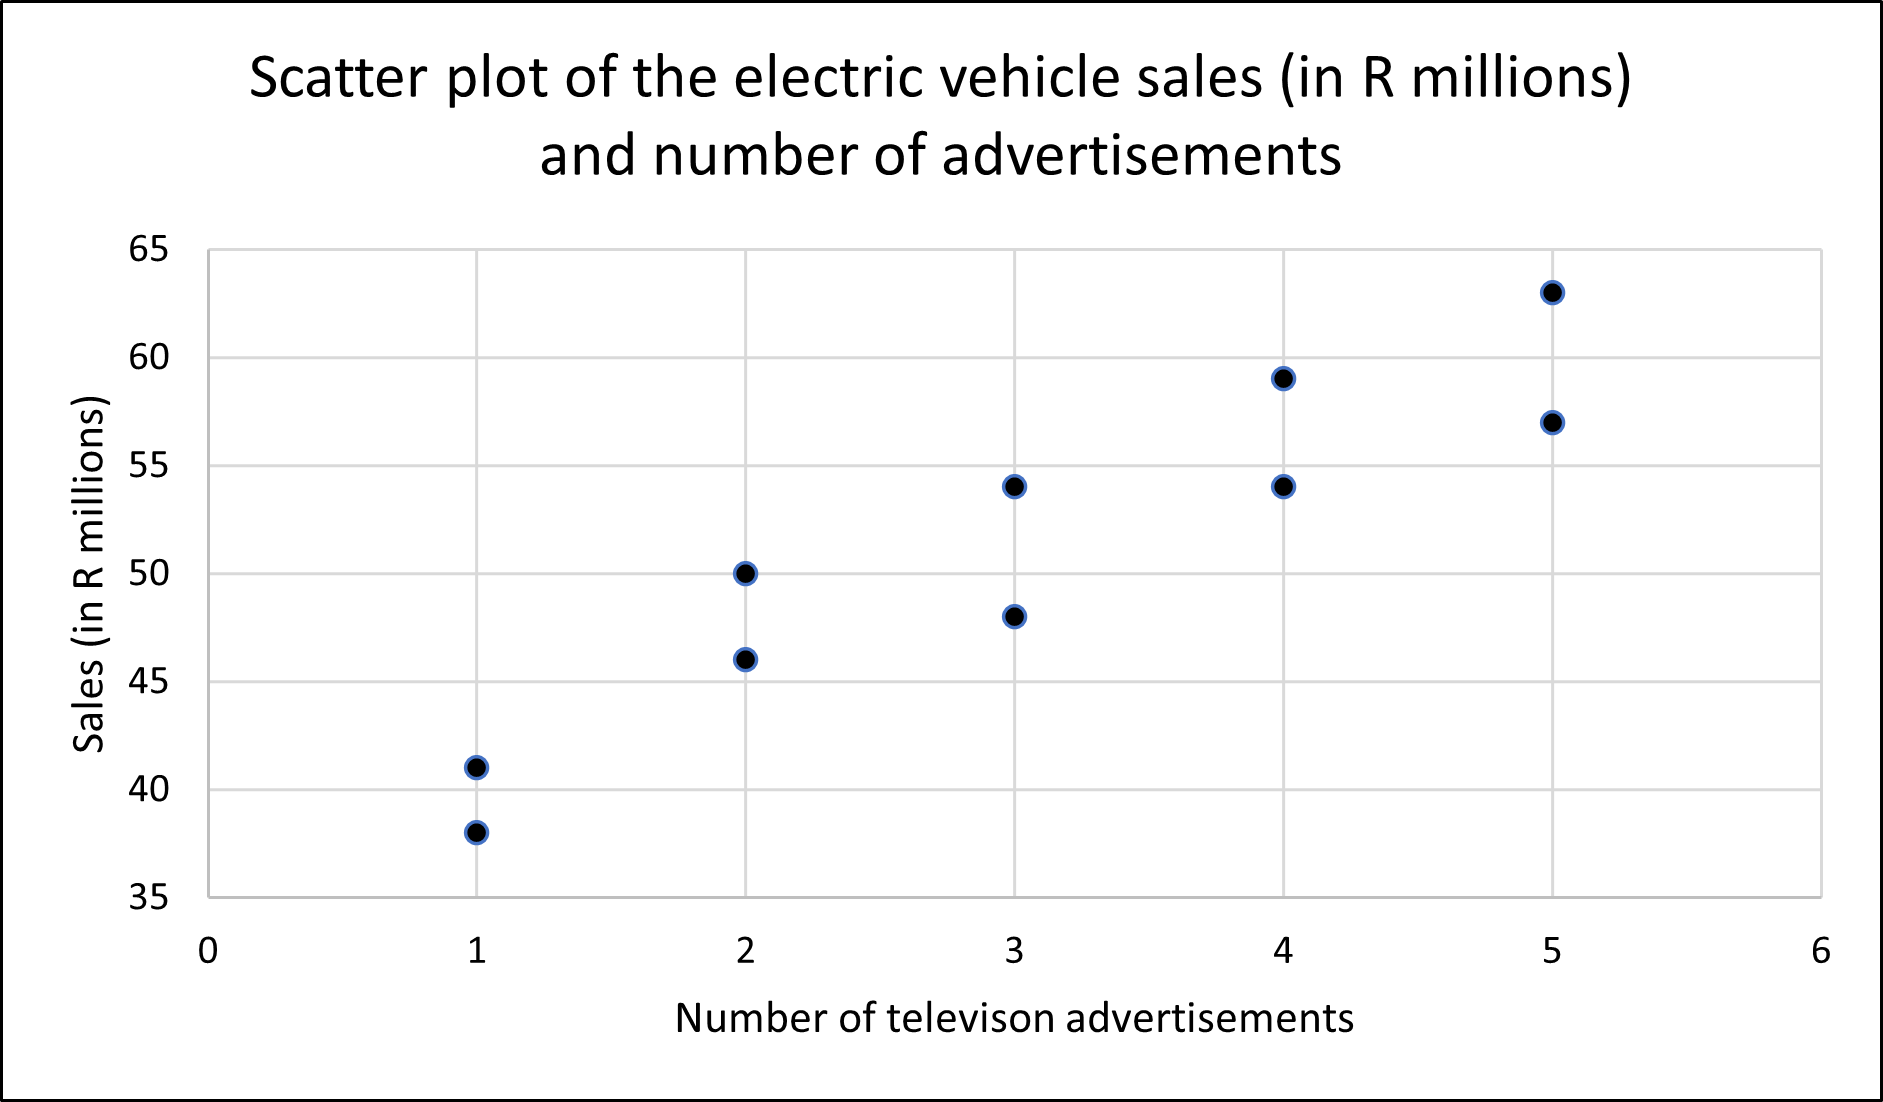
\includegraphics[width=0.8\linewidth]{Figures-Chapter1/Scatter} 

}

\caption{Scatter plot of electric vehicle sales (in R millions) and the number of advertisements}\label{fig:unnamed-chunk-4}
\end{figure}

\begin{itemize}
\tightlist
\item
  \textbf{Educational and knowledge sharing} -- visualizations can simplify complex topics and make information more easily accessible to the general public in order to support education and training.
\end{itemize}

\subsection{Types of data visualizations}\label{types-of-data-visualizations}

The choice of a data visualization tool depends on the purpose of the study and the type of data available.

\begin{enumerate}
\def\labelenumi{\arabic{enumi}.}
\item
  For the purpose of visualizing the distribution of the data, we can make use of a

  \begin{enumerate}
  \def\labelenumii{\alph{enumii}.}
  \item
    \textbf{Frequency distribution} -- show the number of observations in each of several non-overlapping categories or classes for both numerical and categorical data.
  \item
    \textbf{Bar chart} -- to show the frequency distribution for a categorical variable.
  \item
    \textbf{Pie chart} -- to show the relative frequency distribution for a categorical variable.
  \item
    \textbf{Dot plot} -- to show the distribution of a numerical variable over the entire range of the data.
  \item
    \textbf{Histogram} -- to show the frequency distribution of a numerical variable over a set of class intervals.
  \item
    \textbf{Stem-and-Leaf} -- to show the rank order and shape of the distribution of numerical data.
  \item
    \textbf{Box-and-Whisker plot} -- to show the distribution of numerical data using five numbers calculated from the data.
  \end{enumerate}
\end{enumerate}

\begin{enumerate}
\def\labelenumi{\arabic{enumi}.}
\setcounter{enumi}{1}
\item
  For the purpose of identifying whether or not the data has a trend overtime, we make use of a

  \begin{enumerate}
  \def\labelenumii{\alph{enumii}.}
  \tightlist
  \item
    \textbf{Line chart} which can be used to visualize time series data.
  \end{enumerate}
\item
  For the purpose of making comparisons between two or more variables in a data set, we can make us of a

  \begin{enumerate}
  \def\labelenumii{\alph{enumii}.}
  \item
    \textbf{Multiple boxplots} -- to compare the distributions of two or more numerical variables.
  \item
    \textbf{Side-by-side or stacked bar charts} -- to compare two categorical variables.
  \item
    \textbf{Pivot-tables (crosstabulation)} -- to compare the frequency distribution of two categorical distributions.
  \end{enumerate}
\item
  For the purpose of describing the relationship between numerical variables we can make use of

  \begin{enumerate}
  \def\labelenumii{\alph{enumii}.}
  \tightlist
  \item
    \textbf{Scatter plots} to (1) represent the relationship between two numerical variables, (2) identify the type of pattern represented in the scatter plot (linear constant upward or downward trend, curved pattern or no apparent pattern at all); (3), if there is a pattern, determine how strong is the pattern (do all the points follow the pattern exactly or not? In Section \ref{sec1-7}, we will define a numerical measure that can quantify the strength of a linear pattern) and (4) identify if there are any unusual observations (points that are far from the cluster of the majority of the points).
  \end{enumerate}
\item
  For the purpose of displaying geographical data, we can make use of

  \begin{enumerate}
  \def\labelenumii{\alph{enumii}.}
  \item
    \textbf{Heat map} -- to show the intensity or density of a variable across a geographical area using a color gradient. These maps are effective for visualizing, for instance, crime hotspots.
  \item
    \textbf{Flow map} -- to show the direction and magnitude of the movement, migration or flow of people, goods or information between different locations.
  \item
    \textbf{Choropleth map} -- to represent quantitative or qualitative data associated with geographic regions such as countries. In contrast to a heat map, in a choropleth map, the geographic regions are not based on the variable of interest but are chosen based on known spatial information. These maps are effective for visualizing data on, for instance, population density or income levels.
  \item
    \textbf{Cartograms} -- to show the relative influence or importance of different geographical regions based on some quantitative variable such as population size. These visual tools work by distorting the size of the geographical regions by making them proportional to the numerical value of the variable of interest. For instance, geographic regions with larger population sizes will be larger on the map.
  \item
    \textbf{Point maps} -- to show the location of a specific outcome, such as the site of a wildfire, on the map.
  \item
    \textbf{Bubble maps} -- to show the relative magnitude of a specific outcome, such as the impact of a wildfire at a specific location, on the map. The larger the bubble, the higher the impact. ~
  \end{enumerate}
\end{enumerate}

\subsection{Components of a data visualization tool}\label{components-of-a-data-visualization-tool}

In order for a visual summary to effectively communicate the message behind the data, it must possess the following core features:

\begin{itemize}
\item
  An appropriate descriptive title that explains the data being shown.
\item
  Clear labels with the units of measurements and appropriate scales for both the x-axis (horizontal) and y-axis (vertical).
\item
  A legend identifying the different data series, where appropriate.
\end{itemize}

The figure below shows a graph of the 14-day Covid-19 infection rate in the South Africa provinces of Gauteng and Kwa-Zulu Natal for the period 1 December 2020 to 28 February 2021.

\begin{figure}

{\centering 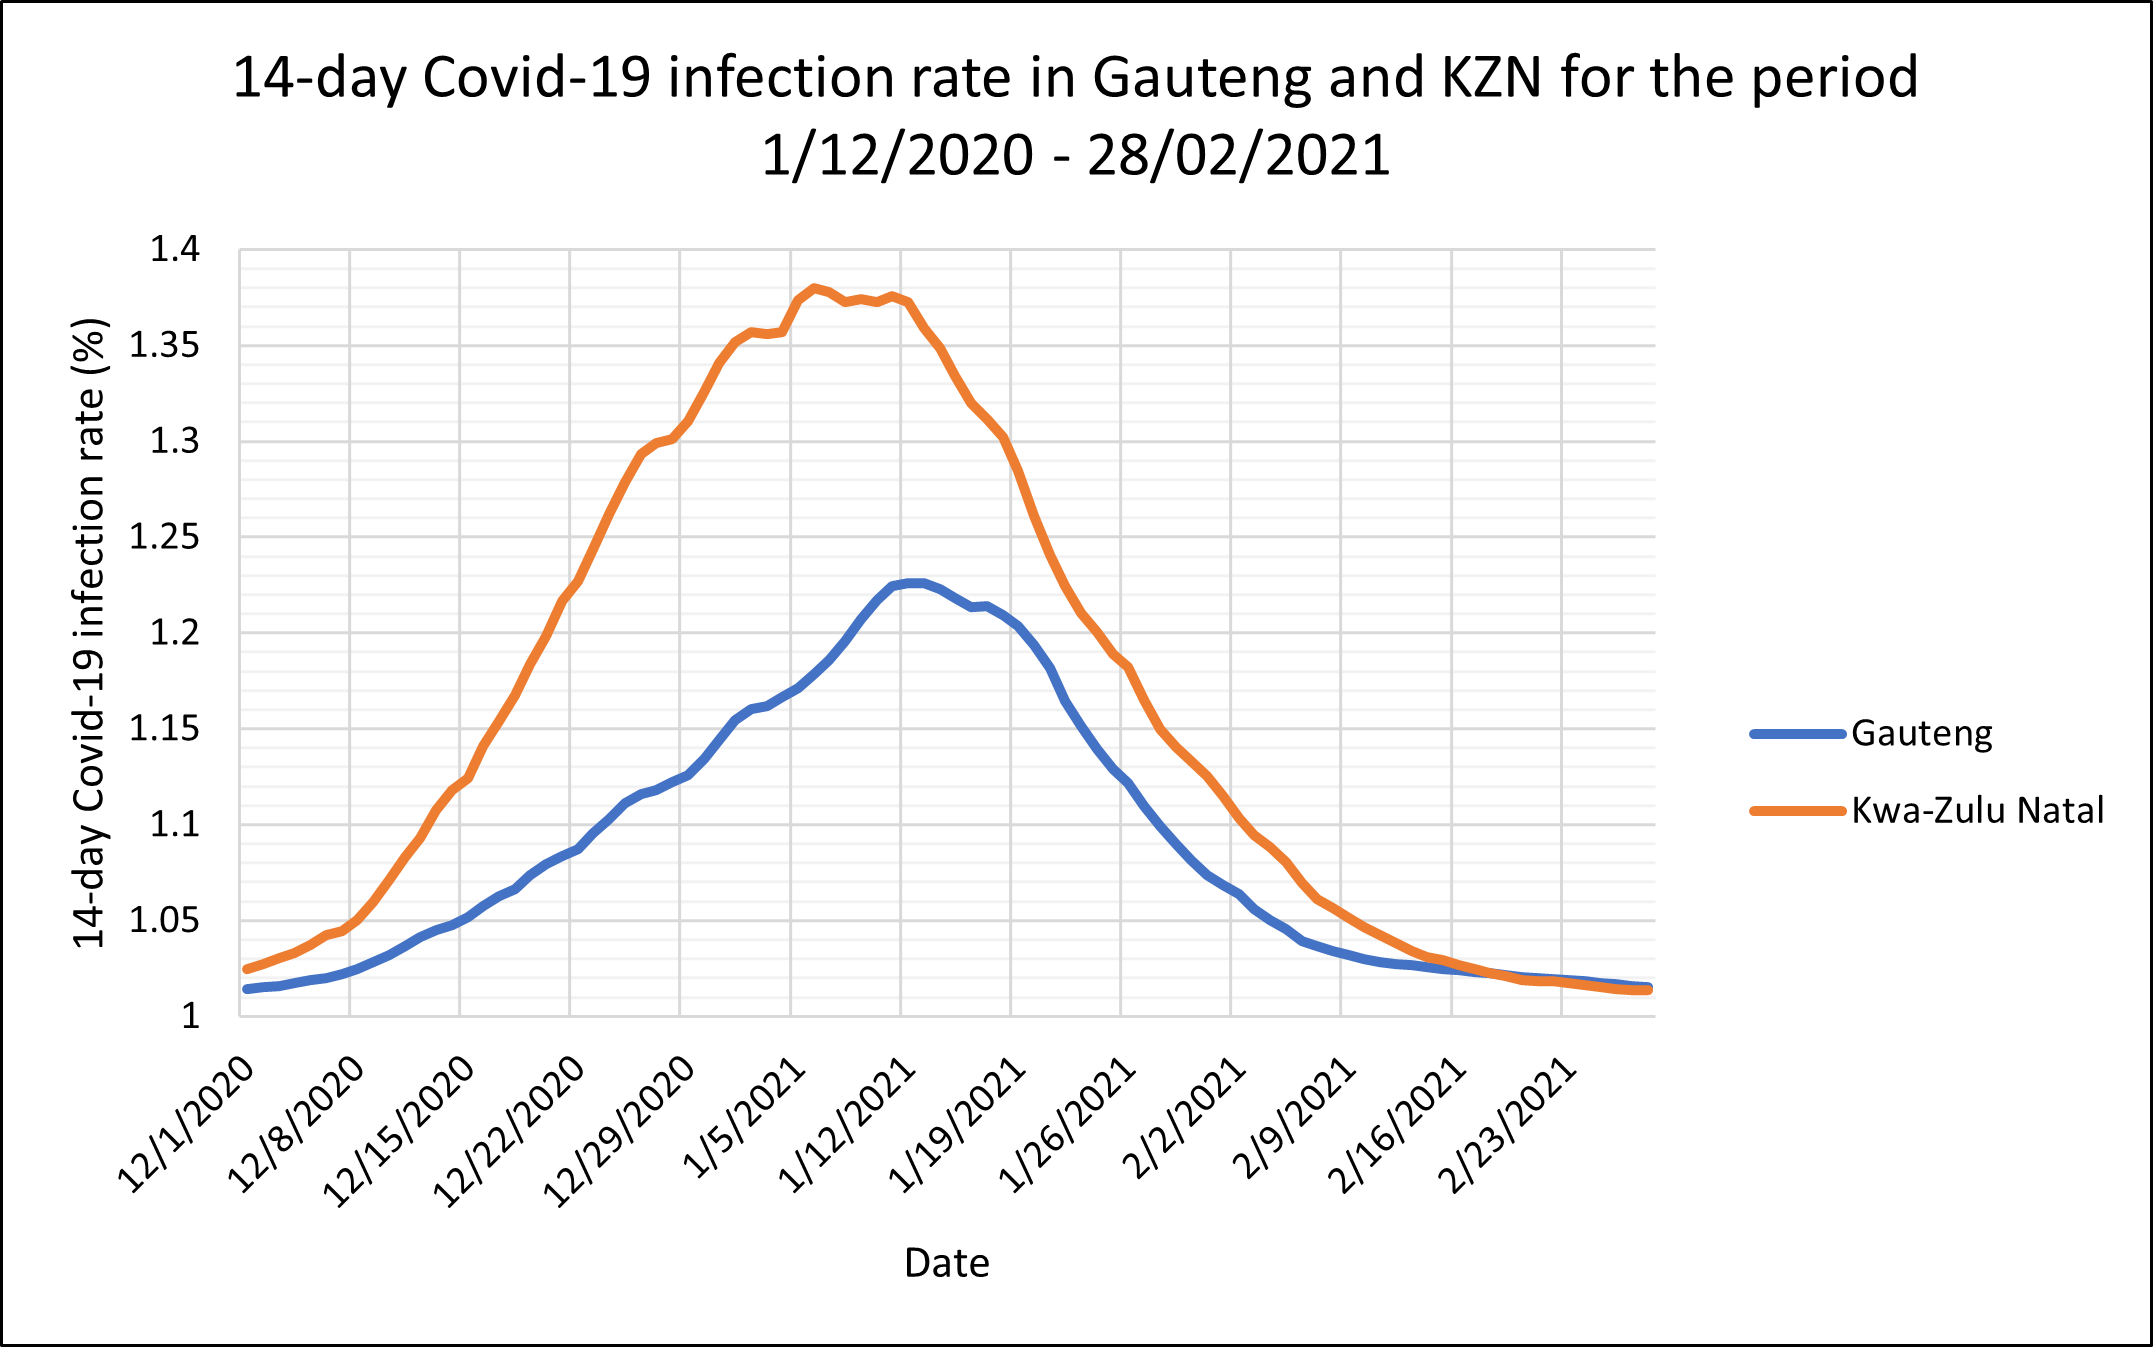
\includegraphics[width=0.7\linewidth]{Figures-Chapter1/Covid-1} 

}

\caption{The 14-day Covid-19 infection rate in the South African provinces of Gauteng and Kwa-Zulu Natal for the period 1 December 2020 to 28 February 2021}\label{fig:covid-1}
\end{figure}

Figure \ref{fig:covid-2} is a copy of Figure \ref{fig:covid-1} highlighting the core features of a graph.

\begin{figure}

{\centering 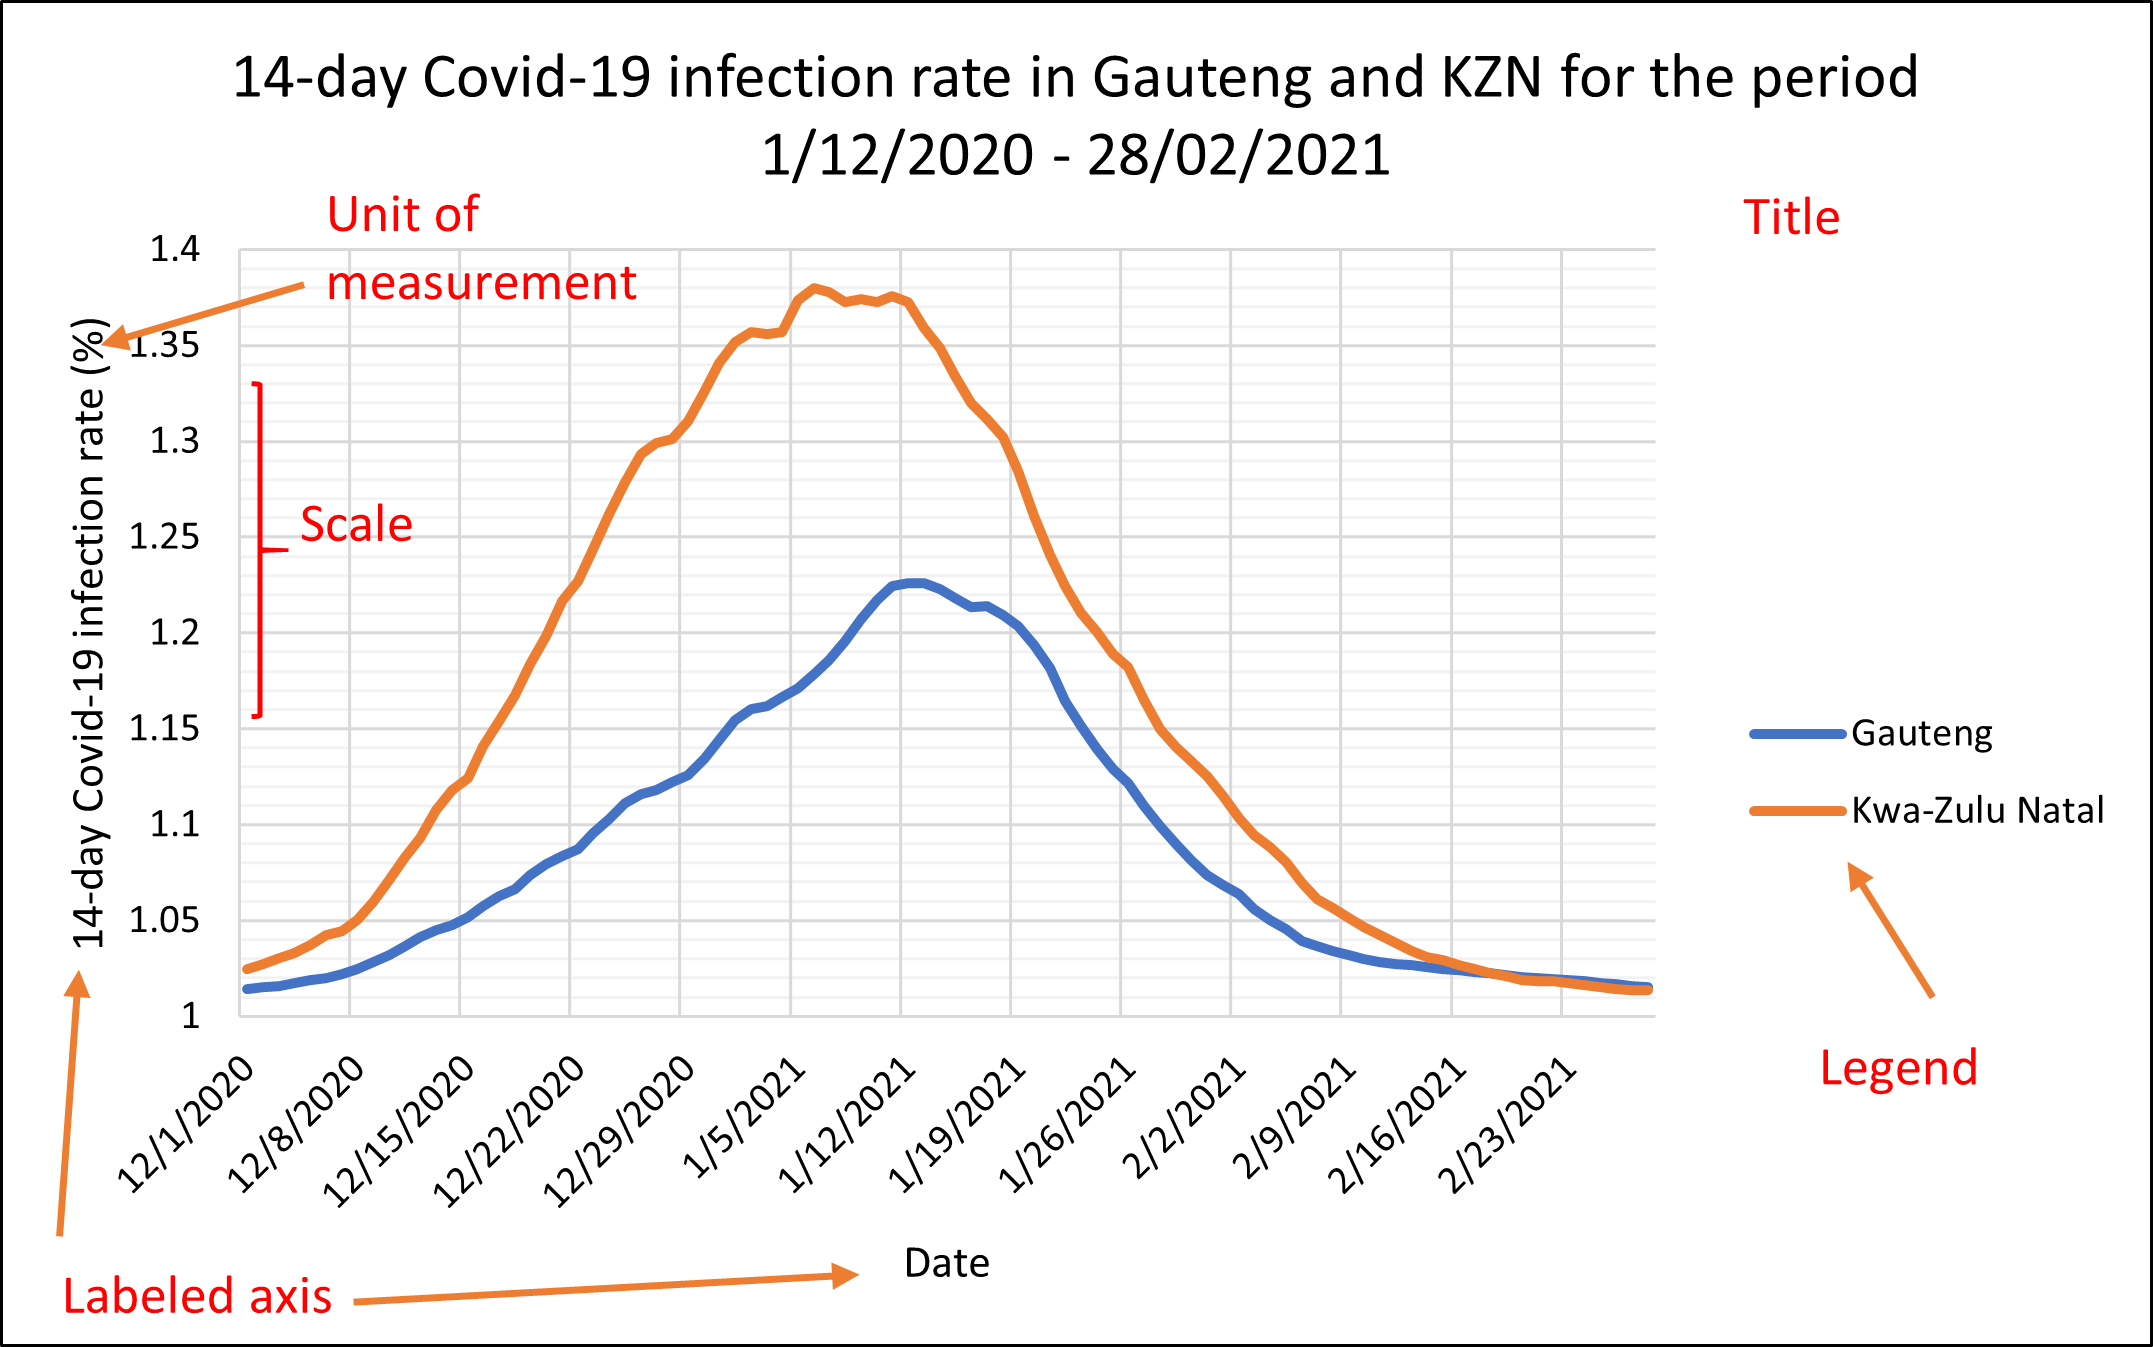
\includegraphics[width=0.7\linewidth]{Figures-Chapter1/Covid-2} 

}

\caption{Same as Figure \\ref{fig:covid-1}}\label{fig:covid-2}
\end{figure}

\subsection{Advantages and Disadvantages of data visualization}\label{advantages-and-disadvantages-of-data-visualization}

Data visualization can be an advantageous skill to have because

\begin{itemize}
\item
  it appeals to any audience which means you can communicate the data to anyone;
\item
  it allows you to communicate efficiently and effectively about data;
\item
  quickly detect patterns or anomalies in the data;
\item
  it facilitates timely decision-making;
\end{itemize}

While there are many obvious advantages to data visualization, there are also some less obvious disadvantages to data visualization such as:

\begin{itemize}
\item
  using the wrong visualization tool;
\item
  concluding from a scatter plot that the observed correlation implies causation;
\item
  making biased conclusions.
\item
  Due to their ease of apprehension, they can often be used to spread misinformation.
\end{itemize}

\subsection{Exercises to Section 1.6}\label{exercises-to-section-1.6}

\textbf{Question 1}

What is data visualization?

\textbf{Question 2}

For each of the following scenarios, specify the appropriate visualization technique (s):

\begin{enumerate}
\def\labelenumi{\alph{enumi}.}
\item
  The City of Tshwane is concerned about income inequality, the mayor wants to investigate the distribution of income.
\item
  In an effort to efficiently allocate police personnel, the City of Johannesburg wants to know which areas have the most criminal incidents.
\item
  The forestry, fisheries and the environment ministry of South Africa wants to compare the greenhouse gas emissions across industries in the primary, secondary and tertiary sector.
\item
  The Western Cape province has noted an increase in the number of people from other parts of South Africa, the administration wants to know what is the province of origin for most of the migrants?
\item
  A botanist wants to understand the effect of temperature on the rate of growth of a plant.
\end{enumerate}

\textbf{Question 3}

For each of the following scenarios, specify whether or not the chosen visualization technique is appropriate, if not, state the reason and specify an appropriate technique:

\begin{enumerate}
\def\labelenumi{\alph{enumi}.}
\item
  A financial analyst uses a pie chart to identify the trend in the rand-dollar exchange rate for the period 2000-2020.
\item
  A psychologist uses a box-and-whisker diagram to identify outliers in terms of IQ.
\item
  A zoologist uses a line chart to compare the territory sizes between male tigers and female tigers.
\item
  A sociologist uses a bar chart to study the relationship between an individual's years of education and their voting frequency.
\end{enumerate}

\textbf{Question 4}

The following is a pie chart of the soft-drink preferences of 50 individuals in South Africa:

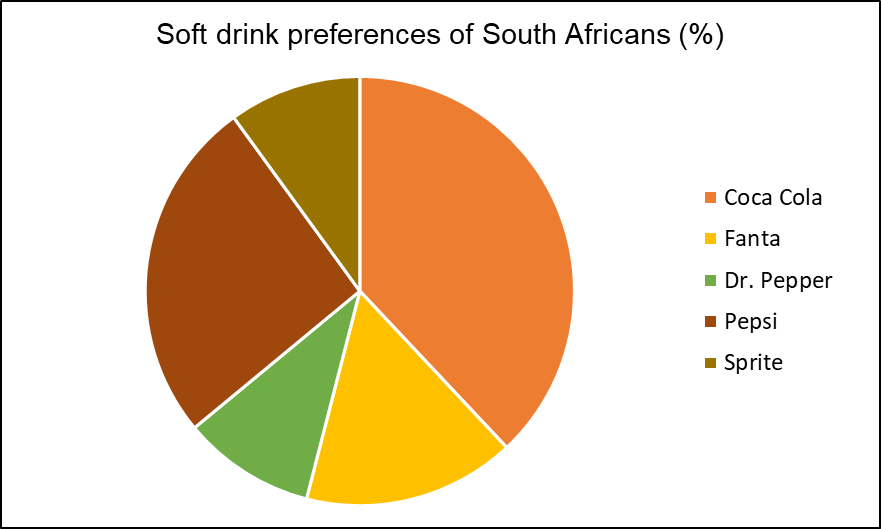
\includegraphics[width=4.16667in,height=\textheight]{images/clipboard-2887671888.png}

Identify what is wrong with the above visualization.

\newpage

\section{Data analysis -- Foundations and Concepts}\label{sec1-7}

Data analysis is the process of systematically using statistical techniques to explore, clean, transform and model data with the purpose of discovering useful information which can then be used to support decision-making.

\subsection{The Data Analysis process}\label{the-data-analysis-process}

Data analysis can be viewed as a sequence of steps combining some of the data literacy skills we have already discussed so far in this book. This process can be summarized as follows:

\begin{enumerate}
\def\labelenumi{\arabic{enumi}.}
\item
  \textbf{Define the study}

  The first and important step in the data analysis process is to clearly define the problem that the analysis aims to address by stating the objectives and specific questions that the analysis aims to answer.
\item
  \textbf{Data collection}

  Once the study is defined, the next step is to collect the relevant data. This can be done using various methods to be discussed in Chapter \ref{ch3}. The choice of method used to collect data depends on the nature of the problem and the questions being asked.
\item
  \textbf{Data cleaning}

  After collecting the data, the next step is to clean the data. This involves identifying and rectify errors, missing values and inconsistencies in the data. Data cleaning will be further discussed and practically demonstrated in Chapter \ref{ch2}.

  \textbf{Note:} The second and third step are part of data management. See Section \ref{sec1-3} for more details.
\item
  \textbf{Data exploration}

  After cleaning the data, we conduct a preliminary analysis to understand the characteristics of the data. See Section \ref{sec1-5} for more details on how this is done in practice.
\item
  \textbf{Data transformation}

  Following from the results of the exploration phase of the data analysis, the data is prepared for analysis by encoding categorical variables, scaling (normalizing or standardizing) some numerical variables and, if necessary, handling outliers.
\item
  \textbf{Data modelling (analysis)}

  Now the data is ready for the actual analysis. This step involves using statistical and mathematical techniques on the data to discover patterns, relationships, similarities or trends.
\item
  \textbf{Interpretation and visualization}

  After the data analysis, the next step is to interpret the obtained results and present them in a manner that can be easily understood. This can be done through visualization.
\end{enumerate}

\subsection{Approaches to Data Analysis}\label{approaches-to-data-analysis}

There are different types of data analysis and each one serves a unique purpose. The choice of which one to use will depend on the nature of your study and what kind of questions you seek to answer.

\begin{enumerate}
\def\labelenumi{\arabic{enumi}.}
\tightlist
\item
  \textbf{Descriptive analysis} is used to describe and summarize the collected data to understand what happened in the past. For example, a university might use descriptive analysis to find out how many first-year students passed last year.
\item
  \textbf{Diagnostic analysis} follows descriptive analysis by going a step further to explain or diagnose why something happened. For example, suppose the number of first years that passed last year dropped significantly, diagnostic analysis can be used to find out why this happened.
\item
  \textbf{Predictive analysis} is used to forecast or predict what might happen in the future based on historical data. For example, a university can use predictive analysis to predict the number of first-year students that will pass next year. In other words, based on what has happened in the past we can find out what could happen in the future.
\item
  \textbf{Prescriptive analysis} is used to make recommendations on what course of action to take in order to reach a desired outcome. For example, suppose a university wants to increase the pass rate for first-year students, a prescriptive analysis might suggest the best course of action towards reaching this outcome.
\end{enumerate}

\subsection{Uses of data analysis in modern society}\label{uses-of-data-analysis-in-modern-society}

Data analysis is a very important data literacy skill that finds application across various fields and domains of application such as:

\begin{itemize}
\item
  \textbf{Marketing research}, where it can be used to assist businesses to understand market trends, consumer preferences and help identify opportunities for product development.
\item
  \textbf{Medical diagnosis}, where it can be used to interpret medical images (e.g.~MRI scans) and also assist in early detection of a disease.
\item
  \textbf{Medical drug discovery}, where it is used by pharmaceutical companies, such as Johnson and Johnson, to develop a drug by conducting clinical trials and testing the effectiveness of the drug.
\item
  \textbf{Fraud detection}, where it can be use by banks to identify unusual transaction patterns and detect fraudulent activities.
\item
  \textbf{Risk management}, where it is used by financial services companies to assess a client's credit risk (i.e.~will they be able to pay back the loan) and model risks in the forex market or stock market.
\item
  \textbf{Quality control}, where it is used to monitor and control the quality of products on the production line.
\item
  \textbf{Social science research}, where it is used to analyze survey data to study overall human behavior and sentiment.
\item
  \textbf{Recommendation systems}, where it used by platforms such as Spotify and Netflix to recommend music or shows that you might like based on the content that you viewed in the past.
\item
  \textbf{Environmental monitoring}, where geographical (remote sensing) data is used to monitor ecological changes such as deforestation, water quality and air pollution.
\end{itemize}

\subsection{Data analysis techniques}\label{data-analysis-techniques}

There are many techniques used in data analysis and each one serves a unique purpose and application. In section {[}Data exploration{]}, we discussed data exploration. This is the most basic technique for data analysis. In this section, we will briefly discuss some of the most commonly used and emerging techniques.

\begin{enumerate}
\def\labelenumi{\arabic{enumi}.}
\item
  \textbf{Correlation analysis}

  Correlation analysis is a technique used to understand the linear relationship between two or more numerical variables. A simple measure that is commonly used to describe this relationship is the \textbf{correlation coefficient}, usually denoted by \(r\). The correlation coefficient is used to quantify the strength of the linear relationship between two numerical variables. The value of \(r\) will always lies between \(-1\) and \(1\). Values close to \(-1\) or \(+1\) indicate a strong linear relationship. The closer the value of \(r\) is to zero, say less than 0.5 or more than -0.5, the weaker the linear relationship. As an example of the use of the correlation coefficient, suppose we want to know the strength of the relationship between a student's matric final mark and their final mark at the end of their first-year of study at a university. Given a correlation coefficient of \(r=0.93\), we can say that there is a strong positive linear relationship between a student's matric final mark and their first-year final mark. In other words, a larger final matric mark is strongly associated with a larger first-year final mark. Finally, please note that correlation measures the linear association between two numerical variables and not necessarily causality. In other words, a high correlation between two variables does not mean changes in one variable will cause changes in the other variable.
\item
  \textbf{Regression analysis}

  Regression analysis is a statistical technique used to understand the dependence of one variable, known as a dependent variable, on one or more other variables, known as independent variables. It is commonly used for predictive analysis. A simple and widely applicable approach to regression analysis is the least squares line. Consider two numerical variables \(x\) and \(y\) which are assumed to follow a straight line pattern. The relationship between \(x\) and \(y\) can be described using a straight line given by the equation
\end{enumerate}

\begin{equation}
y=A+Bx \label{eq:eq1}                                            
\end{equation}

where \(y\) is the dependent variable, assumed to depend on \(x\) known as the independent variable. The term \(A\) is the y-intercept and \(B\) is the slope which represents an increase in \(y\) for every unit-increase in \(x\). For a given sample of \((x,y)\) points, we can obtain an estimate of \eqref{eq:eq1}, given by,

\begin{equation}
\hat{y}=a+bx \label{eq:eq2}                                          
\end{equation}

where \(a\) and \(b\) are estimates of \(A\) and \(B\), respectively, obtained by the method of least squares. Hence, equation \eqref{eq:eq2} is known as the least-squares regression line.

Equation \eqref{eq:eq2} can be used to:

\begin{itemize}
\tightlist
\item
  describe the dependence of \(y\) on \(x\) allowing us to learn more about the process that produces \(y\).
\item
  comment on the type of linear pattern between \(x\) and \(y\) (whether its positive, \(b>0\), negative, \(b<0\), or no pattern exists, \(b=0\)).
\item
  measure the influence that \(x\) has on \(y\) based on the magnitude of the value of \(b\).
\item
  predict the future value of \(y\) for a given value of \(x\).
\end{itemize}

As an example of the use of the least-squares line for regression analysis, consider the least squares line \(\hat{y}=60+5x\) estimated to a data set on student population (in 1000s), \(x\), and quarterly pizza sales (R 1000s), \(y\), for a sample of 10 restaurants located near university campuses. The following points can be made about the fitted least-squares line:

\begin{itemize}
\item
  \(b=5>0\) which implies that as student population, \(x\), increases, quarterly sales increase.
\item
  \(a=60\), which means for a restaurant that is not located close to a university (that is, \(x=0\)), the quarterly sales are \(R60000\).
\end{itemize}

Lastly, we can use the least-squares line to predict the quarterly sales for a given size of the student population. For \(x=16\), representing 16000 students, the quarterly sales are predicted to be \(\hat{y}=60+5(16)=140\) or \(R140000\).

\begin{enumerate}
\def\labelenumi{\arabic{enumi}.}
\setcounter{enumi}{2}
\item
  \textbf{Cluster analysis}

  Cluster analysis is used to group a set of objects or entities in such a way that objects in the same group (or cluster) are more similar than those in other clusters. It is commonly used in recommendation systems and market research to find consumers with similar preferences.
\item
  \textbf{Dimension reduction}

  As implied by the name, this technique is used to reduce a large number of variables into few variables in such a way that the remaining variables capture the maximum possible information from the original variables. It is commonly used in conjunction with some of the already-mentioned techniques such as cluster analysis for medical diagnosis.
\item
  \textbf{Hypothesis testing}

  This technique is used to make inference or statements about population characteristics (such as the mean) using sample data. It is commonly used in the control and monitoring of quality in a production process.
\item
  \textbf{Time series analysis}

  This technique is used for the analysis of time-series data. It is commonly used for predictive analysis and understanding the trend overtime. It is commonly used in forecasting or predictive analysis.
\item
  \textbf{Sentiment analysis}

  This technique is used to extract the emotional tone (negative, positive or neutral) behind text data. It is commonly used to understand customer feedback.
\item
  \textbf{Spatial data analysis}

  This technique is used for the analysis of geographical (remote sensing) data, that is data with a spatial component (e.g.~geographic location represented by coordinates). The most important use of this technique is in disease tracking to identify hotspots.
\end{enumerate}

\subsection{Computational tools and software for data analysis}\label{computational-tools-and-software-for-data-analysis}

Modern data analysis is carried out using sophisticated computational tools and software that cater for different needs and levels of expertise. This includes

\begin{enumerate}
\def\labelenumi{\arabic{enumi}.}
\item
  \textbf{Python}

  Python is the most popular high-level general-purpose programming language that can be used for a variety of tasks including data analysis. It is relatively easy to learn and has a range of libraries (pandas, NumPy and Matplotlib) that make it a favorite data analysis and visualization tool among data analysts and data scientists.
\item
  \textbf{R programming language}

  R is an open source (free software) programming language developed specifically for statistical computing and visualization. Overtime, R has evolved to have a wide set of capabilities such as statistical software development and scientific text editing. It is a popular software among statisticians because it features tools such as hypothesis tests, correlation analysis, regression analysis, among many others. ~
\item
  \textbf{SQL (Structured Query Language)}

  SQL is a language for managing and manipulating data that is sored in databases.

  Note that it is not necessary to know programming in order to do data analysis. The following are the most popular non-programming data analysis tools used in industry:
\item
  \textbf{Excel}

  Microsoft Excel is a spreadsheet that is most widely used for data analysis because it is easier to use. It offers a range of features for data collection (using the Sampling tool), exploration (using the Descriptive Analysis tool), modelling (using the Regression Analysis tool) and visualization (using the Charts tool).
\item
  \textbf{SAS (Statistical Analysis System)}

  SAS is an advanced license-based software developed specifical for statistical data analysis and visualization. It is made up of procedures that can perform tasks such as data exploration (PROC MEANS), hypothesis testing (PROC TTEST) and many others.
\item
  \textbf{Power BI}

  Power BI is a powerful business analytics tool developed by Microsoft. It enables users to create interactive visualizations with self-service business intelligence capabilities. Power BI is used to transform raw data into useful insights that are easy to understand through dashboards and reports.
\item
  \textbf{Tableau}

  Tableau is a business analytics tool used to create interactive and shareable dashboards that show trends, variations and densities for important day-to-day business metrics through charts and graphs.
\end{enumerate}

\subsection{Exercises to Section 1.7}\label{exercises-to-section-1.7}

\textbf{Question 1}

For each of the following case studies, specify which type of data analysis is appropriate:

a. Eskom wants to reduce overall electricity waste and improve the stability of the national electricity grid. To achieve this, they want to propose energy-saving strategies to its customers.

b. Absa has noticed a decrease in their corporate clients overtime. They want to know what could be behind this.

c. In order to inform her decision on many warm clothing to bring on her trip to Essen, Germany in January, Renate wants to know what the average temperature will be in Essen, Germany in January.

d. In order to inform their decision on the interest rate at their next meeting, the South African Reserve Bank wants to know what the inflation rate will be in the next 12 months {[}predictive{]}.

e. A general practitioner (GP) wants to know how many COVID-19 patients she treated between 2020 -- 2022.

\textbf{Question 2}

For each of the following case studies, specify which data analysis tool (s) is/are appropriate:

a. Given past data on electricity consumption, Eskom wants to determine the amount of electricity that will be consumed in the next winter season.

b. A plant physiologist wants to understand dependence of plant growth on factors such as water availability, temperature and soil nutrient levels.

c. Suppose that you want to study the response of a plant to changes in temperature, drought, salinity.

d. A biochemist wants to classify proteins with similar structural characteristics.

e. The World Health Organization (WHO) wants to identify geographic hotspots for the monkeypox disease.

f. The WHO wants to understand public opinion about a new strain of virus from social media posts.

g. In order to inform their decision on the interest rate, the South African Reserve Bank (SARB) wants to forecast the average value of the rand per US dollar in the next 12 months.

\chapter{Sources and types of data}\label{ch2}

Add content here.

\chapter{Data Handling in Excel}\label{ch3}

In this chapter, you will be introduced to some of the fundamental skills needed to work with data in Excel. Excel is a powerful tool enabling us to organise, analyse and visualise data efficiently. This chapter will not only enhance your ability to manage data but also lay the foundation for the more advanced data analysis.

Topics covered in this chapter includes:

\begin{itemize}
\item
  Data importing
\item
  Data cleaning
\item
  Data manipulation
\end{itemize}

\section{Data importing}\label{data-importing}

In this subsection, the focus is on importing data into Excel from different sources such that we can start working with it. This is a crucial first step when doing data analysis.

\subsection{Change decimal separator settings in Excel}\label{change-decimal-separator-settings-in-excel}

On most devices, the default setting in Excel is to use a comma as a decimal separator. This causes some difficulties especially when working with .csv (comma separated value) files.

\newpage

\begin{enumerate}
\def\labelenumi{\arabic{enumi}.}
\tightlist
\item
  Go to the \textbf{File} tab.
\end{enumerate}

\begin{center}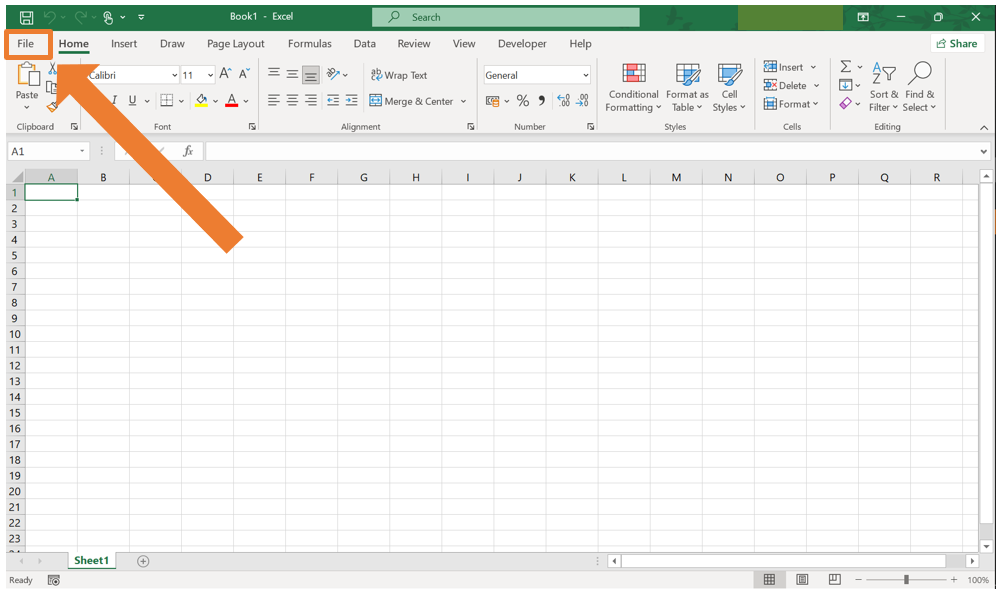
\includegraphics[width=0.6\linewidth]{Figures/decimal_step1} \end{center}

\begin{enumerate}
\def\labelenumi{\arabic{enumi}.}
\setcounter{enumi}{1}
\tightlist
\item
  At the bottom of the menu at the left, select \textbf{More\ldots{}} and then \textbf{Options}.
\end{enumerate}

\begin{center}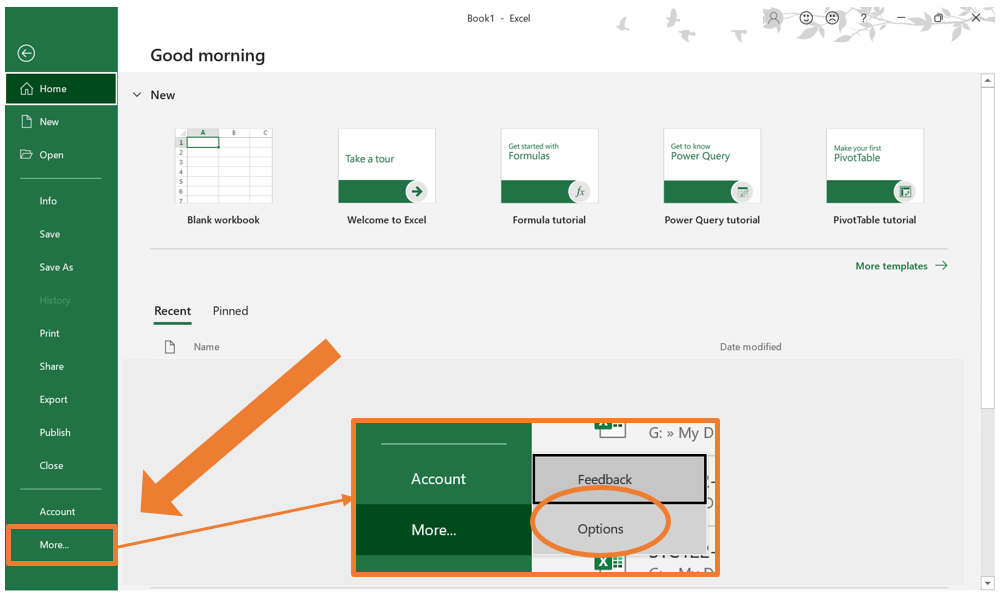
\includegraphics[width=0.6\linewidth]{Figures/Decimal_step2} \end{center}

\begin{enumerate}
\def\labelenumi{\arabic{enumi}.}
\setcounter{enumi}{2}
\tightlist
\item
  The Excel Options window will open. Select \textbf{Advanced} on the menu at the left.
\end{enumerate}

\begin{center}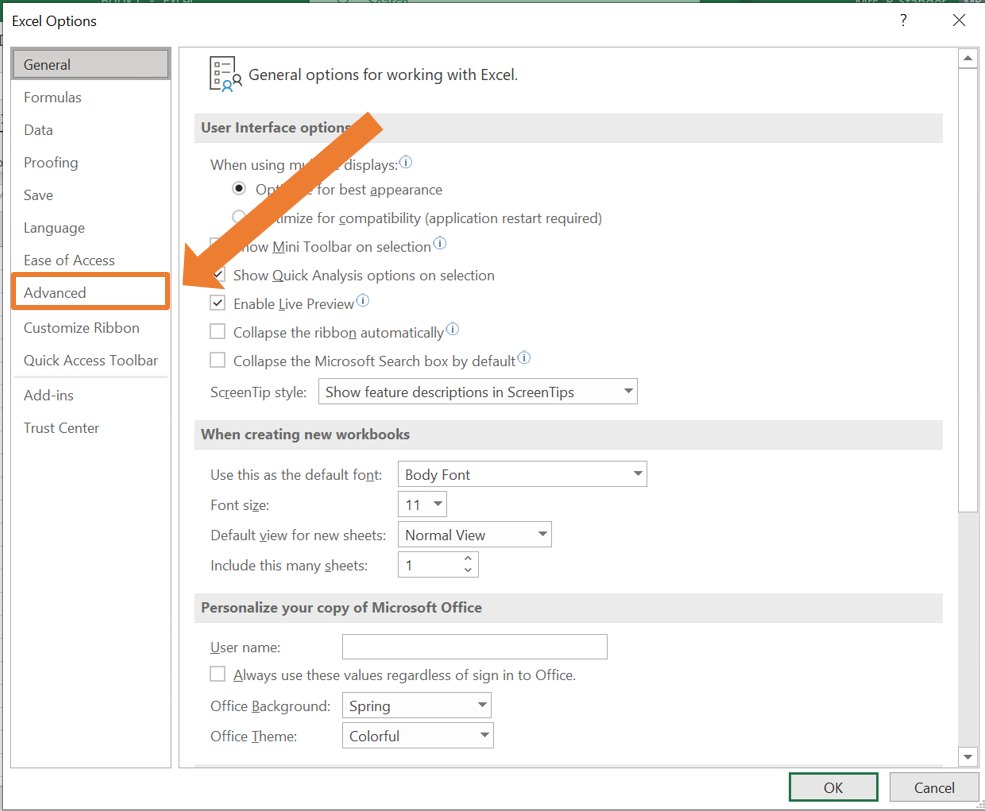
\includegraphics[width=0.6\linewidth]{Figures/Decimal_step3} \end{center}

\begin{enumerate}
\def\labelenumi{\arabic{enumi}.}
\setcounter{enumi}{3}
\tightlist
\item
  Under \textbf{Editing Options} there is a you can specify the \textbf{Decimal separator}. In the box, make sure to have a full stop (\texttt{.}) instead of a comma (\texttt{,}).
\end{enumerate}

\begin{center}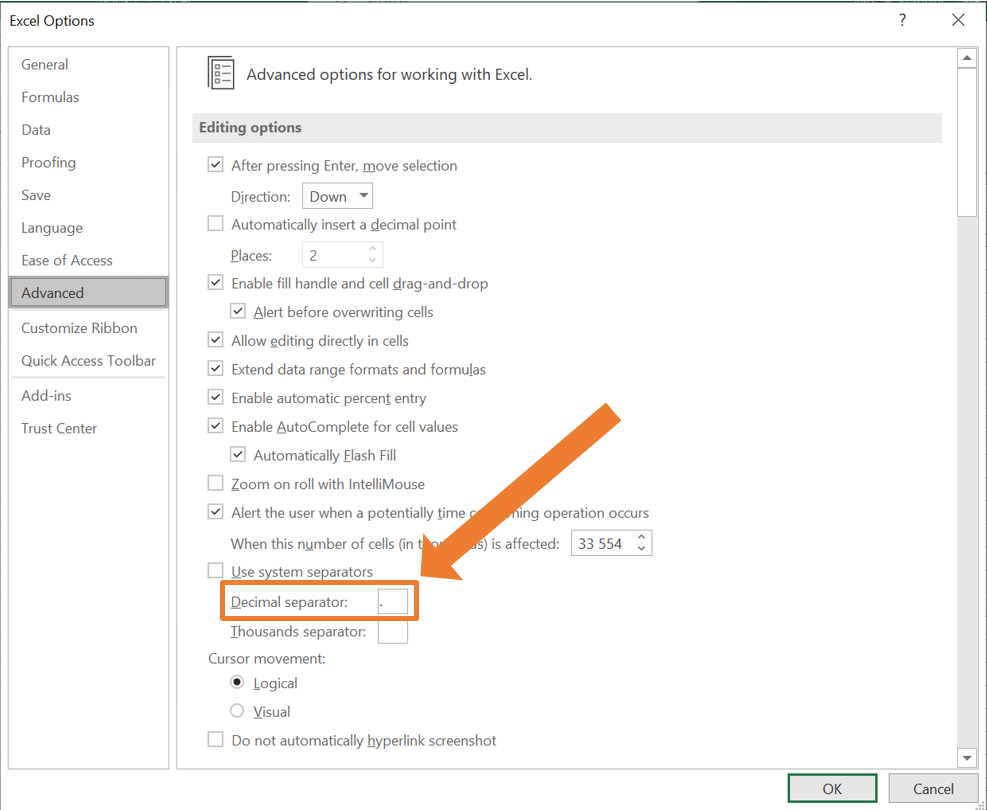
\includegraphics[width=0.6\linewidth]{Figures/Decimal_step4} \end{center}

\begin{enumerate}
\def\labelenumi{\arabic{enumi}.}
\setcounter{enumi}{4}
\tightlist
\item
  Click \textbf{OK} to save the changes.
\end{enumerate}

\subsection{Opening a .xlsx file in Excel}\label{opening-a-.xlsx-file-in-excel}

A file with the \texttt{.xlsx} extension is a standard Excel file. Such files can be opened in Excel effortlessly. The following steps can be followed:

\begin{enumerate}
\def\labelenumi{\arabic{enumi}.}
\tightlist
\item
  Go to the \textbf{File} tab.
\end{enumerate}

\begin{center}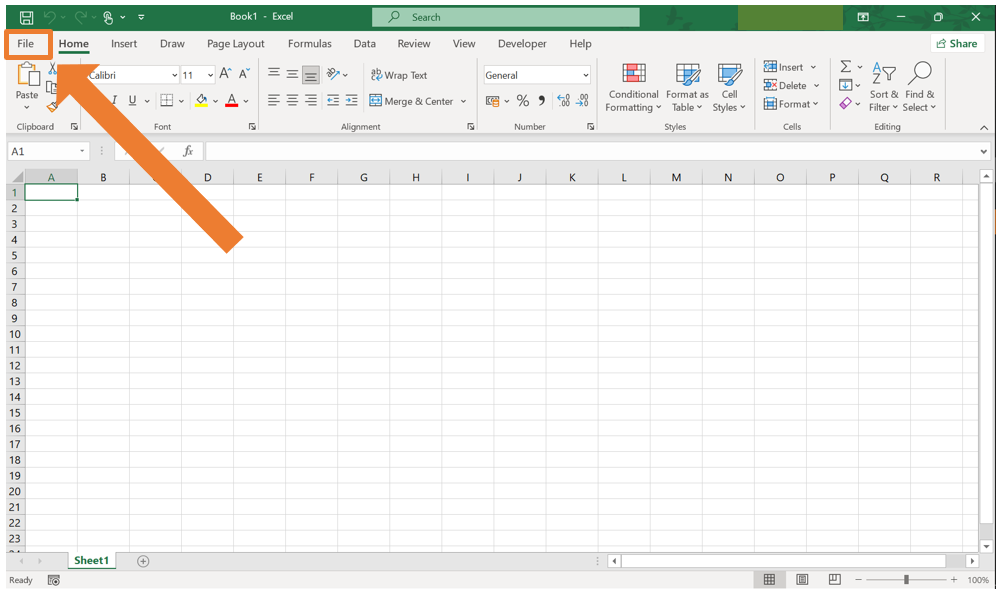
\includegraphics[width=0.6\linewidth]{Figures/decimal_step1} \end{center}

\newpage

\begin{enumerate}
\def\labelenumi{\arabic{enumi}.}
\setcounter{enumi}{1}
\tightlist
\item
  Select \textbf{Open}.
\end{enumerate}

\begin{center}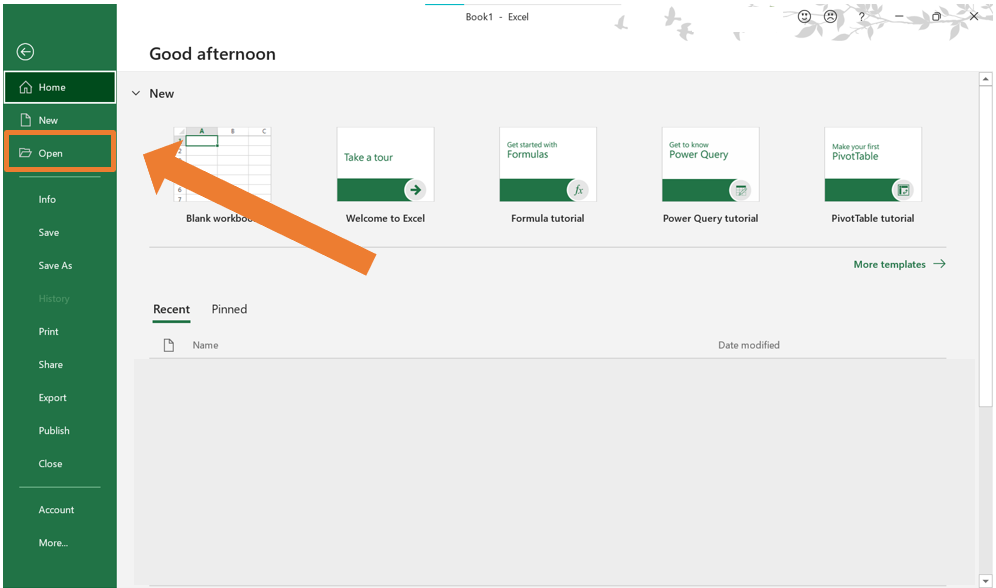
\includegraphics[width=0.6\linewidth]{Figures/import_open_1} \end{center}

\begin{enumerate}
\def\labelenumi{\arabic{enumi}.}
\setcounter{enumi}{2}
\tightlist
\item
  Click on \textbf{Browse}.
\end{enumerate}

\begin{center}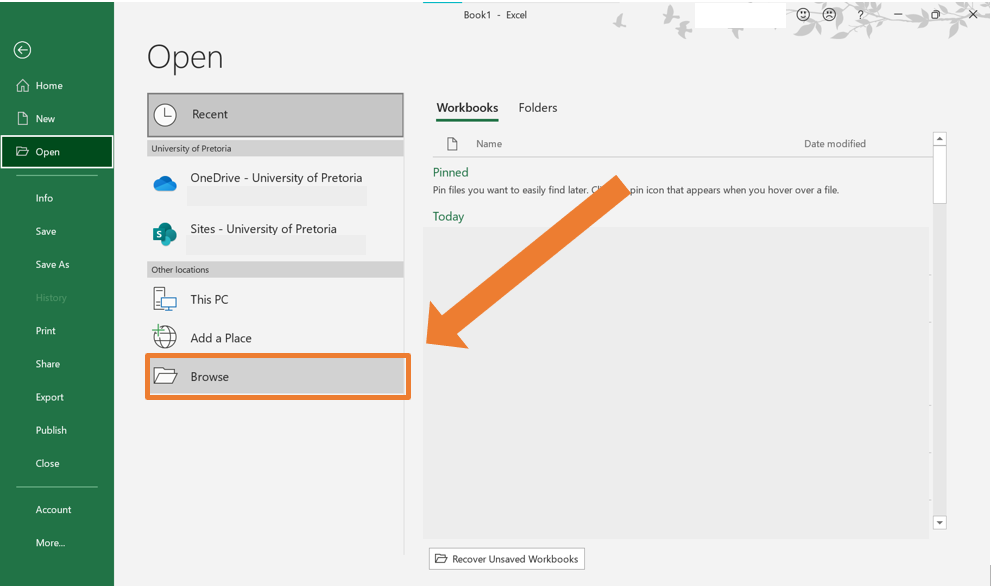
\includegraphics[width=0.6\linewidth]{Figures/import_open_2} \end{center}

\begin{enumerate}
\def\labelenumi{\arabic{enumi}.}
\setcounter{enumi}{3}
\tightlist
\item
  Navigate to the location of the file you want to import and select it.
\end{enumerate}

\subsection{Importing a .txt file in Excel}\label{importing-a-.txt-file-in-excel}

Some external programs can export data in a text (\texttt{.txt}) file. If you wish to do some data manipulation or work with the data in any other way, you will need to import the text file in Excel.

When data is stored in a text file, various symbols (known as delimiters) are used to indicate the separation between columns. These delimiters help structure the data so that tools like Excel or programming languages can interpret it accurately. Here's an explanation of common delimiters used in text files:

\newpage

\begin{enumerate}
\def\labelenumi{\arabic{enumi}.}
\tightlist
\item
  Tabs
\end{enumerate}

\begin{center}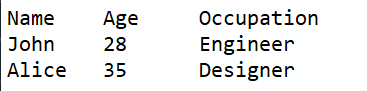
\includegraphics[width=0.4\linewidth]{Figures/import_tabs} \end{center}

\begin{enumerate}
\def\labelenumi{\arabic{enumi}.}
\setcounter{enumi}{1}
\tightlist
\item
  Commas
\end{enumerate}

\begin{center}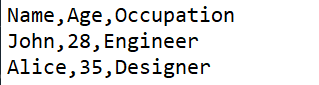
\includegraphics[width=0.4\linewidth]{Figures/import_commas} \end{center}

\begin{enumerate}
\def\labelenumi{\arabic{enumi}.}
\setcounter{enumi}{2}
\tightlist
\item
  Semicolons
\end{enumerate}

\begin{center}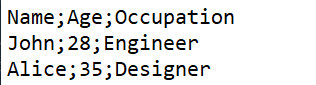
\includegraphics[width=0.4\linewidth]{Figures/import_semicolon} \end{center}

\begin{enumerate}
\def\labelenumi{\arabic{enumi}.}
\setcounter{enumi}{3}
\tightlist
\item
  Pipes
\end{enumerate}

\begin{center}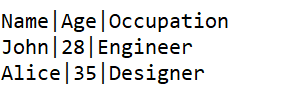
\includegraphics[width=0.4\linewidth]{Figures/import_pipes} \end{center}

\subsubsection{Example}\label{example}

You have obtained access to a data set available exclusively in text format, named \texttt{SACensus2022-Data-Text.txt}. To work with this data set, you need to import it into Excel. Follow these steps to complete the process:

\begin{enumerate}
\def\labelenumi{\arabic{enumi}.}
\tightlist
\item
  Open Excel and navigate to the \textbf{Data} tab. In the \textbf{Get/Transform Data} group click the \textbf{From Text/CSV} button.
\end{enumerate}

\begin{center}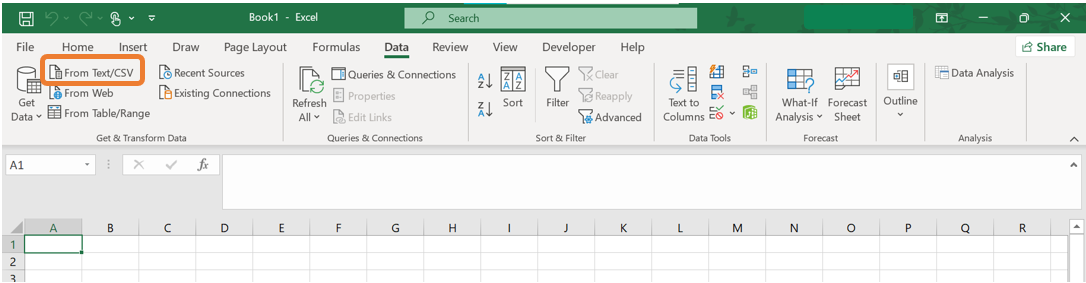
\includegraphics[width=0.7\linewidth]{Figures/import_1} \end{center}

\newpage

\begin{enumerate}
\def\labelenumi{\arabic{enumi}.}
\setcounter{enumi}{1}
\tightlist
\item
  A file selection window will appear. Navigate to the location of the file you want to import and select it. By default, the dropdown menu at the bottom right will show ``Text Files (\texttt{.txt}, \texttt{.csv})'' as the file type. Ensure this option is selected.
\end{enumerate}

\begin{center}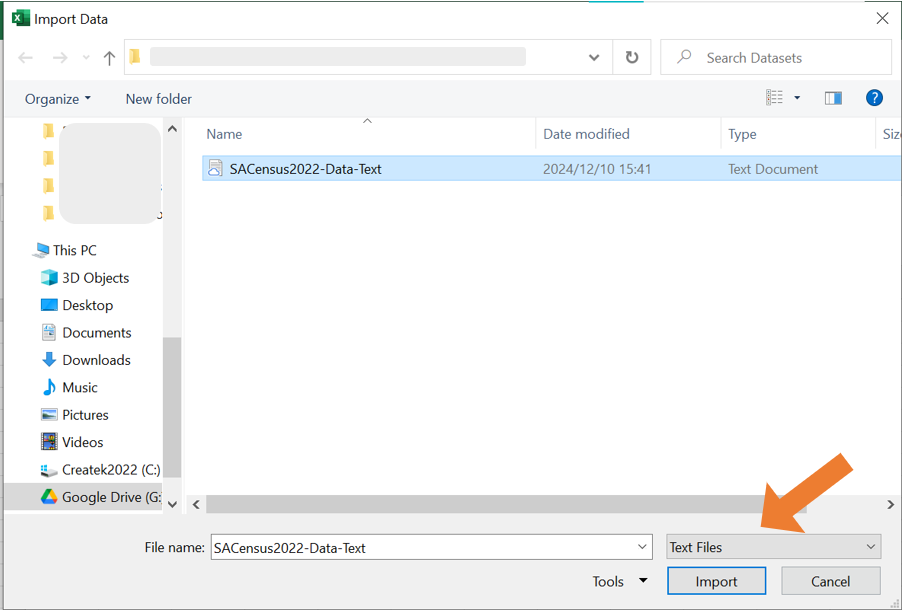
\includegraphics[width=0.6\linewidth]{Figures/import_2} \end{center}

\begin{enumerate}
\def\labelenumi{\arabic{enumi}.}
\setcounter{enumi}{2}
\tightlist
\item
  The Import Wizard will open in Excel. Check that the data columns are separated correctly. Excel typically detects the delimiter (e.g., commas, tabs) automatically, but you can change it using the dropdown menu at the top of the wizard if needed.
\end{enumerate}

\begin{center}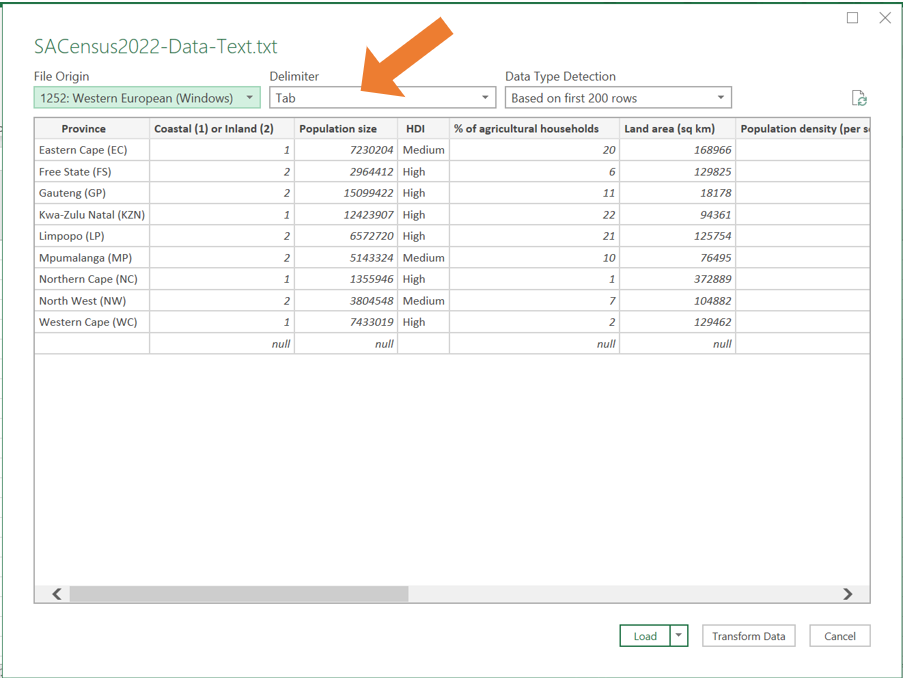
\includegraphics[width=0.7\linewidth]{Figures/import_3} \end{center}

\newpage

\begin{enumerate}
\def\labelenumi{\arabic{enumi}.}
\setcounter{enumi}{3}
\tightlist
\item
  Click \textbf{Load} to import the data into a new worksheet. The data will now be displayed in Excel, ready for use.
\end{enumerate}

\begin{center}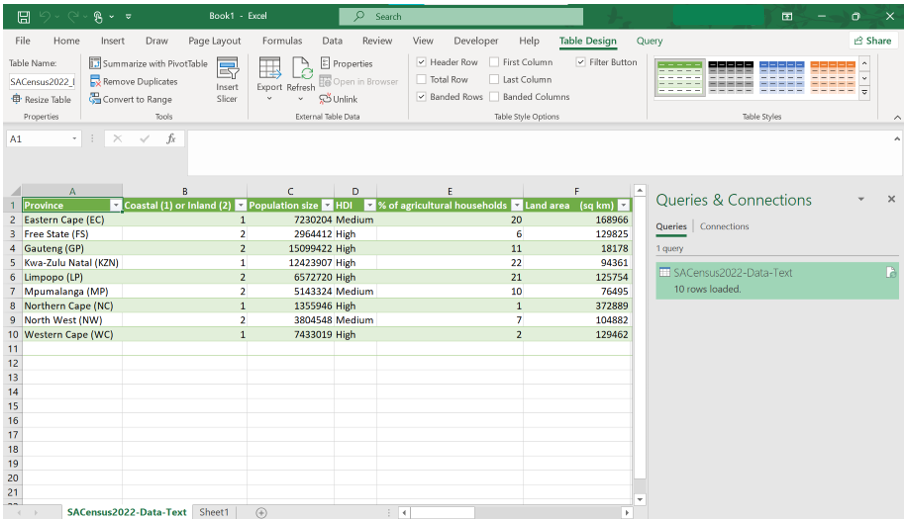
\includegraphics[width=0.7\linewidth]{Figures/import_4} \end{center}

\textbf{NOTE:} The same process can be followed to open a \texttt{.csv} file in Excel. In the case where the settings for the decimal separator is correct, a \texttt{.csv} file can be opened using \textit{File > Open > Browse} and selecting the desired file.

\subsection{Importing data from a website}\label{importing-data-from-a-website}

It is also possible to import a data table into Excel directly from a website, saving you the effort to manually retype the information you need.

Suppose you need to compile a list of all the districts in South Africa. You found such a list on Wikipedia and want to import it into Excel. Follow these steps:

\begin{enumerate}
\def\labelenumi{\arabic{enumi}.}
\tightlist
\item
  Open Excel and navigate to the \textbf{Data} tab. In the \textbf{Get \& Transform Data} group click the \textbf{From Web} button.
\end{enumerate}

\begin{center}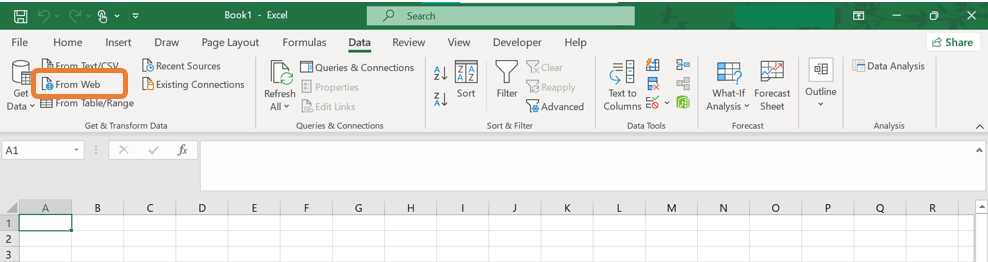
\includegraphics[width=0.7\linewidth]{Figures/web_1} \end{center}

\newpage

\begin{enumerate}
\def\labelenumi{\arabic{enumi}.}
\setcounter{enumi}{1}
\tightlist
\item
  In the \textbf{From Web} wizard, paste the URL of the website containing the table you want to import, then click \textbf{OK}.
\end{enumerate}

\begin{center}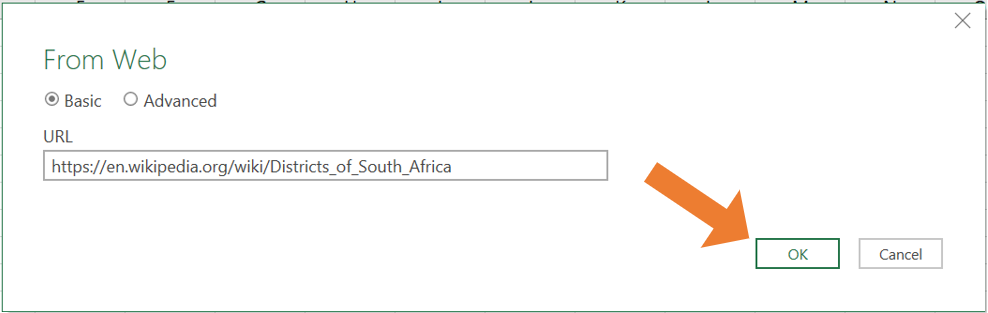
\includegraphics[width=0.6\linewidth]{Figures/web_2} \end{center}

\begin{enumerate}
\def\labelenumi{\arabic{enumi}.}
\setcounter{enumi}{2}
\tightlist
\item
  Next the \textbf{Navigator} window will open. On the left-hand side, you will see a list of tables available from the webpage. Click on a table name to preview the contents of the table on the right-hand side. Select the correct table you want to import. Click on \textbf{Load} to import the table into your Excel worksheet.
\end{enumerate}

\begin{center}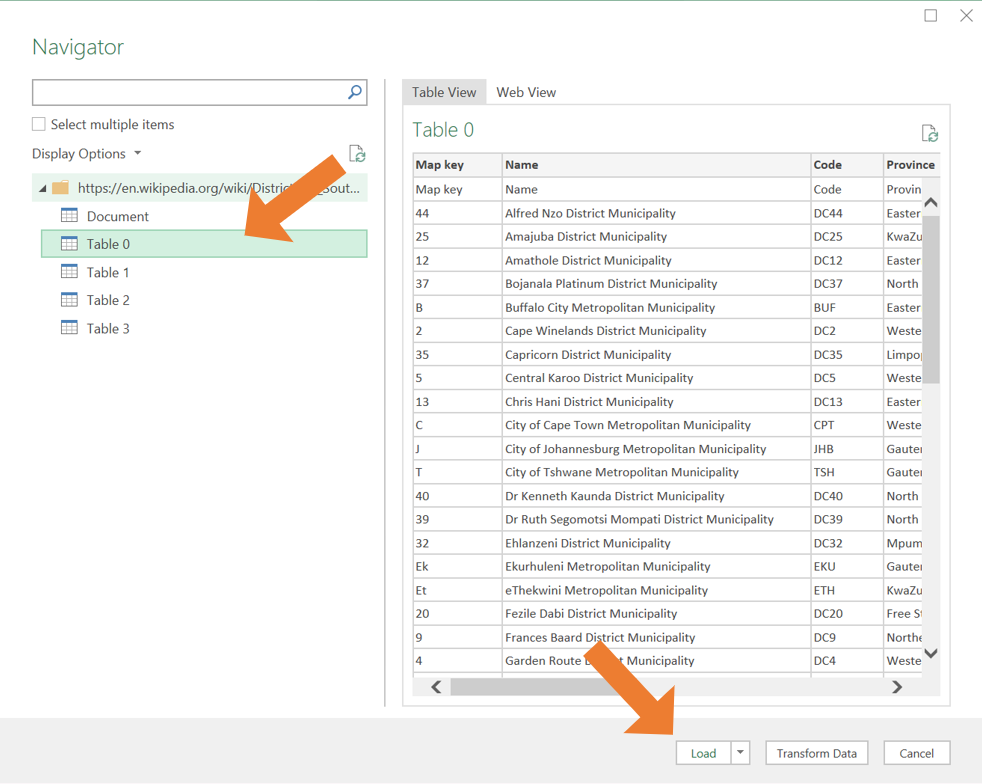
\includegraphics[width=0.7\linewidth]{Figures/web_3} \end{center}

Alternatively, the \textbf{From Web} wizard can be accessed using the \textbf{GetData} button in the \textbf{Get \& Transform Data} group.

\begin{center}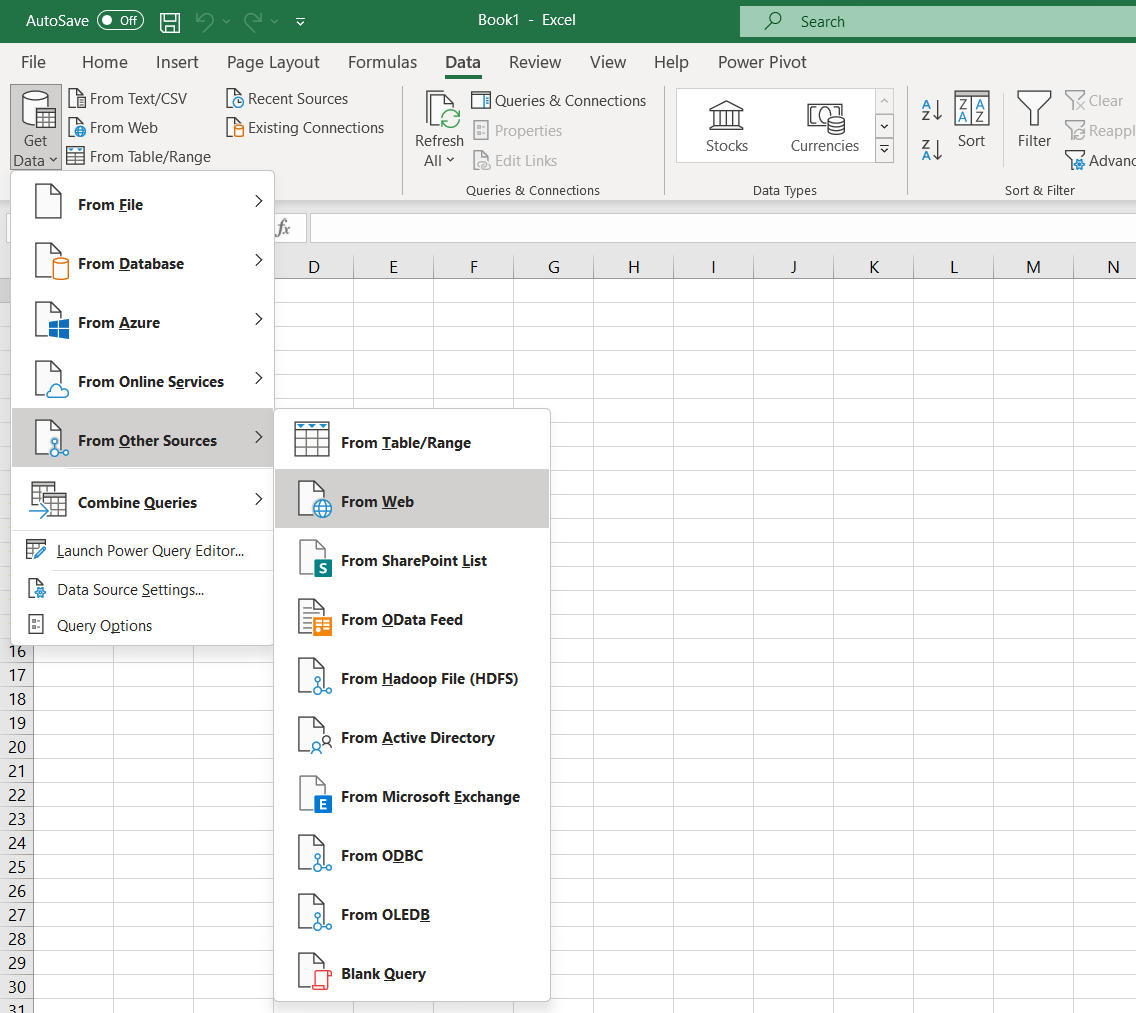
\includegraphics[width=0.6\linewidth]{Figures/Section3-1} \end{center}

\section{Data cleaning}\label{data-cleaning}

Data cleaning is an essential process of identifying and correcting inconsistencies and inaccuracies within a dataset. This process improves the quality, accuracy and reliability for the data. In fact, a data analyst spends a lot of time on preparing the data for analysis. It is very rare that the raw data is in the correct format and without any errors.

Data cleaning is the process of transforming raw data into consistent data that can be analysed.

To ensure that the data set is cleaned and refined before starting an analysis is crucial to assure that the analysis is accurate and therefore that better-informed decisions can be deduced from the analysis. When statistical analysis is performed on data that isn't properly cleaned, the integrity of the results and findings are compromised and not trustworthy.

Therefore, the analysis is only as reliable as the data that is used for the analysis, making data cleaning an essential step.

The specific data cleaning techniques that one will use always depends on the application at hand and the analysis needed. Here is a list of some data cleaning techniques:

\begin{itemize}
\item
  Removing the data that is not necessary for your analysis.
\item
  Identifying and removing observations that are duplicated.
\item
  Correcting typing errors, errors in capitalisations or inconsistent naming conventions.
\item
  Removing or imputing missing data.
\item
  Encoding categorical data either to or from a numerical format.
\item
  Ensuring that the data is in a consistent format.
\end{itemize}

\subsection{Example: Data cleaning in Excel}\label{example-data-cleaning-in-excel}

You are given a data set containing information on employees working at Orion Sales. This data set is named \texttt{orion\_sales\_staff.xlsx}. Once you have opened the data set in Excel, you come across some problems with the data set that requires data cleaning.

\begin{center}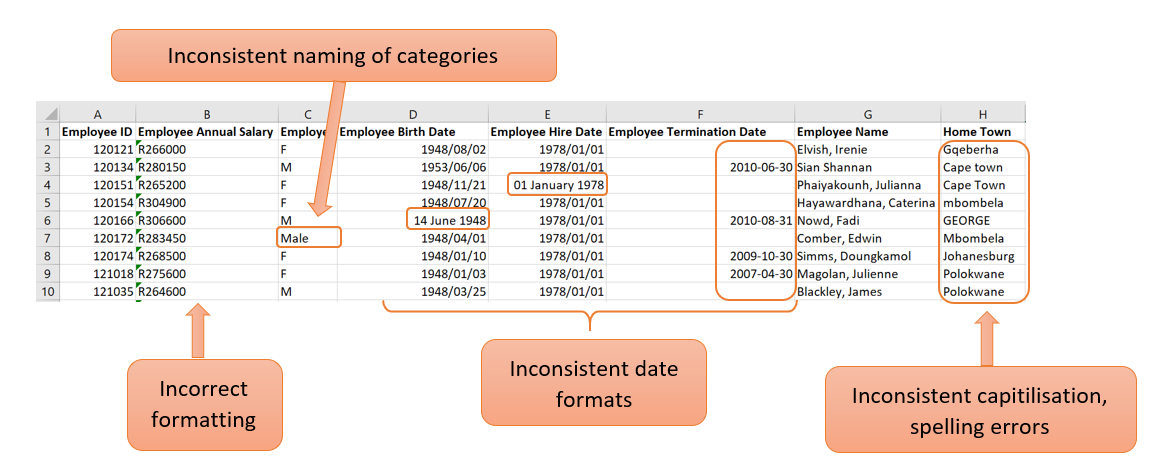
\includegraphics[width=0.7\linewidth]{Figures/cleaning_overview} \end{center}

\subsubsection*{Correct the formatting of a cell}\label{correct-the-formatting-of-a-cell}

In the example above, the values in the ``Employee Annual Salary'' column are seen as text. This is clearly visible with the left alignment of the values in the cell. Because annual salary is a numerical value, the formatting needs to be corrected so that Excel can handle the values as numbers.

This can be corrected with the following steps:

\begin{enumerate}
\def\labelenumi{\arabic{enumi}.}
\tightlist
\item
  If you click in the cell, there will be a yellow block with an exclamation mark on the left.
\end{enumerate}

\begin{center}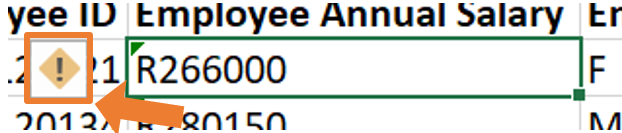
\includegraphics[width=0.4\linewidth]{Figures/cleaning_formatting_1} \end{center}

\begin{enumerate}
\def\labelenumi{\arabic{enumi}.}
\setcounter{enumi}{1}
\tightlist
\item
  By clicking on the warning sign, a dropdown list will open where you can choose the option ``Convert to Number''.
\end{enumerate}

\begin{center}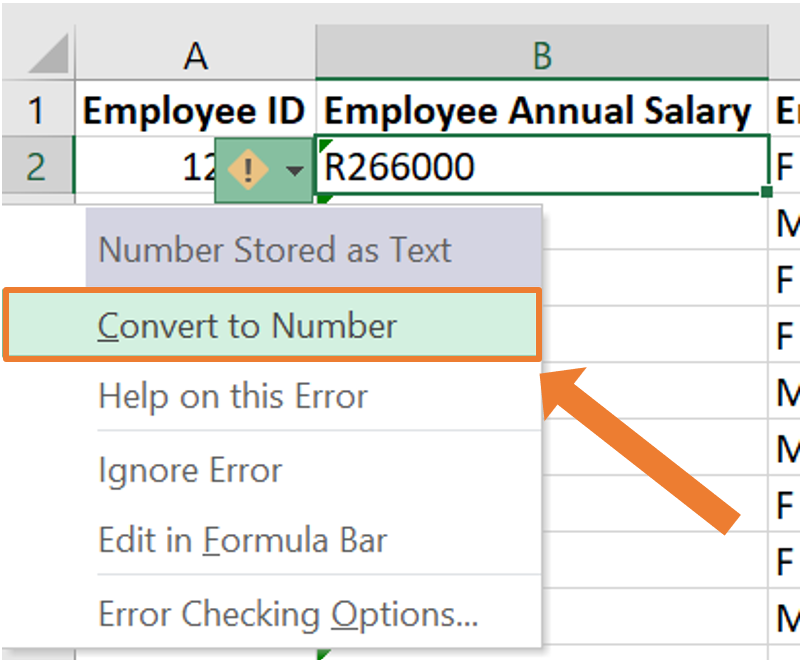
\includegraphics[width=0.4\linewidth]{Figures/cleaning_formatting_2} \end{center}

\begin{enumerate}
\def\labelenumi{\arabic{enumi}.}
\setcounter{enumi}{2}
\tightlist
\item
  Now the cell's formatting will be corrected. This can be seen by the value being right aligned within the cell.
\end{enumerate}

\begin{center}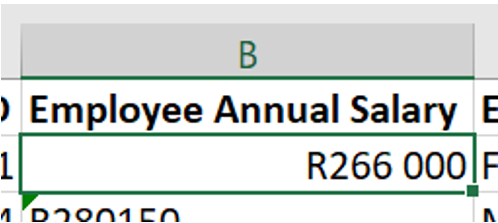
\includegraphics[width=0.4\linewidth]{Figures/cleaning_formatting_3} \end{center}

\begin{enumerate}
\def\labelenumi{\arabic{enumi}.}
\setcounter{enumi}{3}
\tightlist
\item
  To do this for an entire column, The same procedure can be followed by highlighting all the cells that need to be changed.
\end{enumerate}

This process will automatically change the format of the cells from text to ``currency''. If you work with this data set in Excel, this formatting will be sufficient as Excel knows how to work with this. If the data set is imported into another statistical program (which you will be familiarised later on), the format of this column needs to be ``Number'' instead of ``Currency''.

This can be done by navigating to the ``Number'' group on the Home tab in Excel and opening the dropdown list. From this dropdown list, the appropriate formatting can be selected which is ``Number'' in this case.

\begin{center}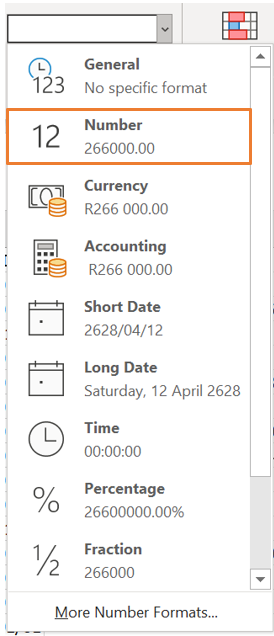
\includegraphics[width=0.4\linewidth]{Figures/cleaning_formatting_4} \end{center}

\subsubsection*{Inconsistent naming of categories}\label{inconsistent-naming-of-categories}

In column C of the example above, the categories are not named consistently. This column consists of the gender of each employee. By glancing at the screenshot of the first few lines of the data, it can be seen that the categories are labelled as ``M'' (for male) and ``F'' (for female). However, in line 7, the entry is ``Male''. There can be more occurrences like this further in the data. Having inconsistent naming of categories is not ideal as this will cause problems when you start to work with the data. For example, when constructing frequency tables or barplots.

This can be corrected with the following steps:

\begin{enumerate}
\def\labelenumi{\arabic{enumi}.}
\tightlist
\item
  Select all the columns of the data set. In the ``Editing'' group on the ``Home'' tab, click on ``Sort \& Filter'' and then on ``Filter. This will allow you to filter the data by a specific column.
\end{enumerate}

\begin{center}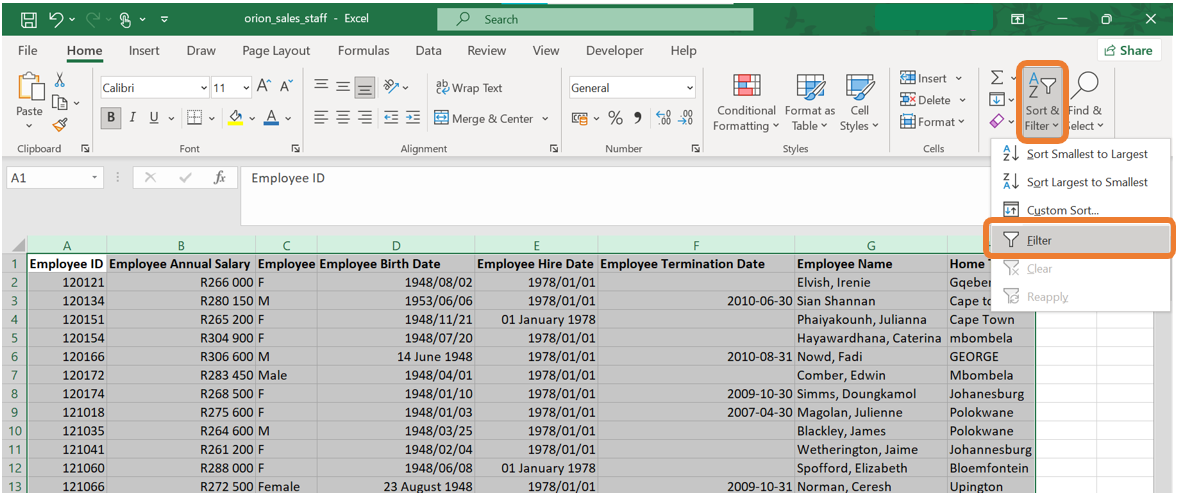
\includegraphics[width=0.7\linewidth]{Figures/cleaning_categories_1} \end{center}

\begin{enumerate}
\def\labelenumi{\arabic{enumi}.}
\setcounter{enumi}{1}
\tightlist
\item
  The filter icon will now be next to each column name. When clicking on the item next to the column name you would like to filter on, a menu will open up. On this menu, you have the ability to sort the data by this column or filter certain categories. In the screenshot below, all the categories are ticked meaning that all the observations of the data set will be displayed. In the example below, it can be seen that there are categories named ``M'', ``F'', ``Male'' and ``Female''. We would like to change all the observations with category ``Female'' to ``F'' and all the observations with category ``Male'' to ``M''.
\end{enumerate}

\begin{center}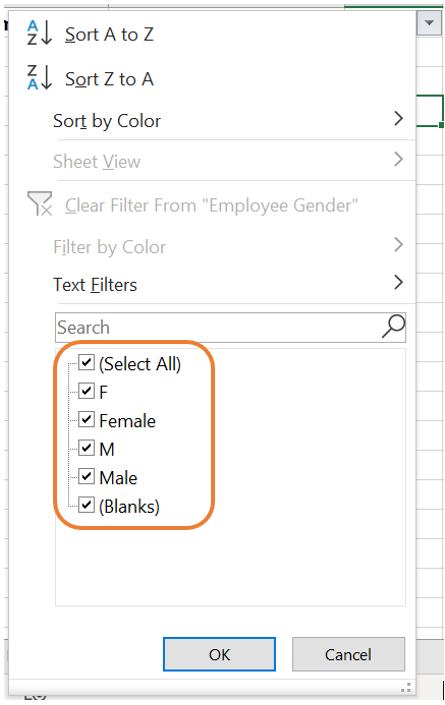
\includegraphics[width=0.4\linewidth]{Figures/cleaning_categories_2} \end{center}

\begin{enumerate}
\def\labelenumi{\arabic{enumi}.}
\setcounter{enumi}{2}
\tightlist
\item
  When removing the tick marks of all the categories except one, only the observations from the specific category will be displayed. In our case, let us first filter all the observations where the gender is indicated as ``Female''.
\end{enumerate}

\begin{center}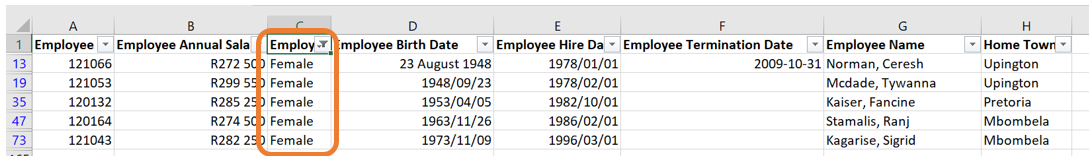
\includegraphics[width=0.7\linewidth]{Figures/cleaning_categories_3} \end{center}

\begin{enumerate}
\def\labelenumi{\arabic{enumi}.}
\setcounter{enumi}{3}
\tightlist
\item
  Having all the observations filtered out, you can manually change the categories to ``F''.
\end{enumerate}

\begin{center}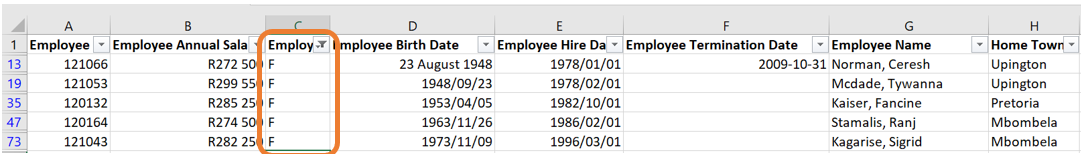
\includegraphics[width=0.7\linewidth]{Figures/cleaning_categories_4} \end{center}

\begin{enumerate}
\def\labelenumi{\arabic{enumi}.}
\setcounter{enumi}{4}
\tightlist
\item
  The came can be done for the males. Again, click on the filter icon next to the column name. Remove the tick marks of all the categories except the one with ``Male''.
\end{enumerate}

\begin{center}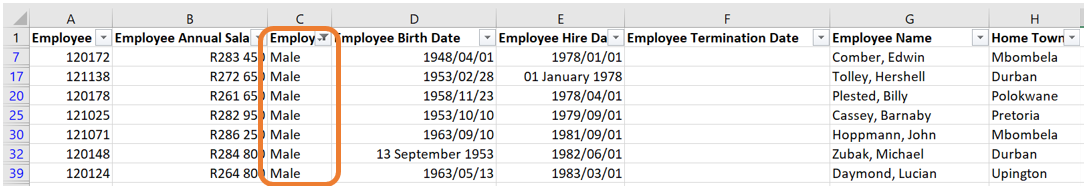
\includegraphics[width=0.7\linewidth]{Figures/cleaning_categories_5} \end{center}

\begin{enumerate}
\def\labelenumi{\arabic{enumi}.}
\setcounter{enumi}{5}
\tightlist
\item
  Then, manually change the categories to ``M''.
\end{enumerate}

\begin{center}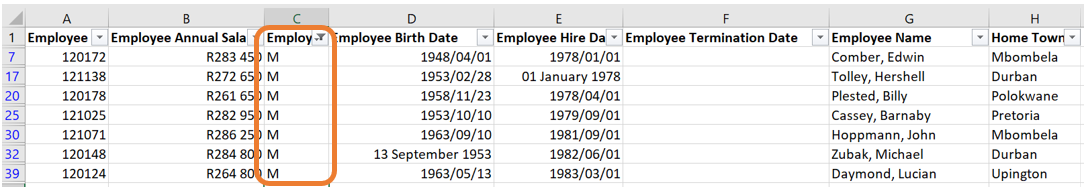
\includegraphics[width=0.7\linewidth]{Figures/cleaning_categories_6} \end{center}

\subsubsection*{Inconsistent capitalisations}\label{inconsistent-capitalisations}

In the column named ``Home Town'', there are a few observations where the name of the town is written in all capital letters, all small letters or the second word is written with a small letter instead of a capital letter.

The best and quickest way to correct this is to create a new column and use built-in Excel functions to do the correction. Let us call this column ``Home Town cleaned''.

Next, we will introduce three new functions that will alter how the names of the towns are written.

\newpage

\begin{enumerate}
\def\labelenumi{\arabic{enumi}.}
\tightlist
\item
  The first function is \texttt{=UPPER()}. This function will return the word in the selected cell written in all capital letters.
\end{enumerate}

\begin{center}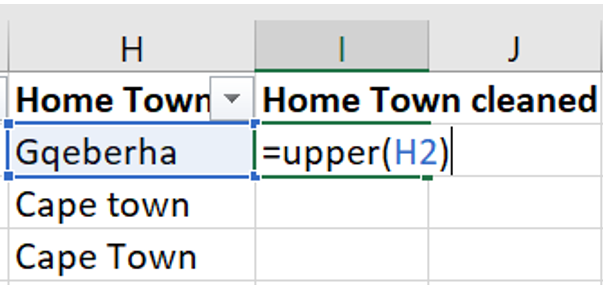
\includegraphics[width=0.4\linewidth]{Figures/capitals_1} \end{center}

\begin{center}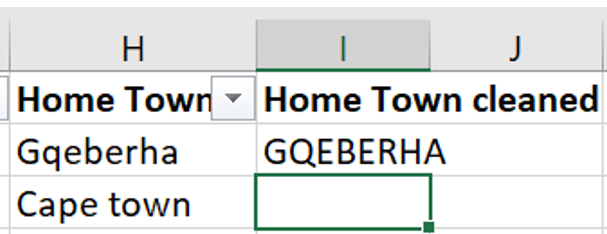
\includegraphics[width=0.4\linewidth]{Figures/capitals_2} \end{center}

\begin{enumerate}
\def\labelenumi{\arabic{enumi}.}
\setcounter{enumi}{1}
\tightlist
\item
  The second function is \texttt{=LOWER()}. This function will return the word in the selected cell written in all lower case letters.
\end{enumerate}

\begin{center}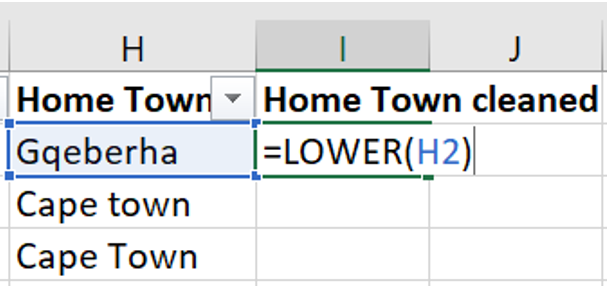
\includegraphics[width=0.4\linewidth]{Figures/capitals_3} \end{center}

\begin{center}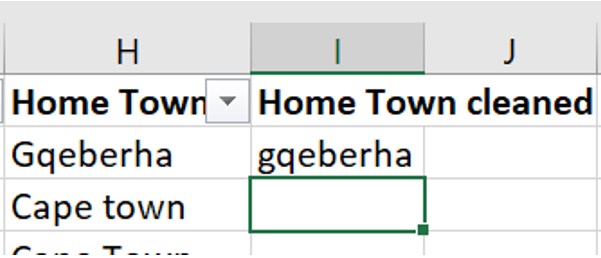
\includegraphics[width=0.4\linewidth]{Figures/capitals_4} \end{center}

\begin{enumerate}
\def\labelenumi{\arabic{enumi}.}
\setcounter{enumi}{2}
\tightlist
\item
  The third function is \texttt{=PROPER()}. This function will return the word in the selected cell where the first letter of each word is written in a capital letter followed by lower case letters.
\end{enumerate}

\begin{center}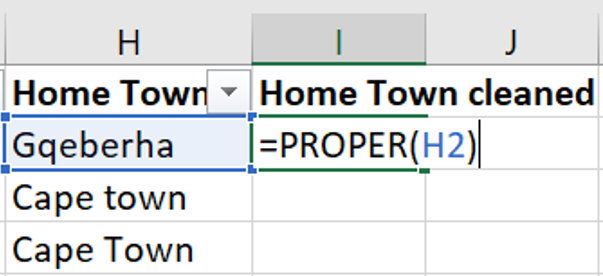
\includegraphics[width=0.4\linewidth]{Figures/capitals_5} \end{center}

\begin{center}\includegraphics[width=0.4\linewidth]{Figures/capitals_6} \end{center}

In the same column, some of the town names are misspelled. This can be corrected similarly to how you corrected the inconsistencies in the category names.

\subsubsection*{Correcting the date format}\label{correcting-the-date-format}

The columns ``Employee Birth Date'', ``Employee Hire Date'' and ``Employee Termination Date'' are examples of columns containing dates.

The dates can be corrected by selecting all the columns containing dates, then selecting the ``short date'' format on the drop-down list in the ``Number'' group on the ``Home tab.

\begin{center}\includegraphics[width=0.4\linewidth]{Figures/dates} \end{center}

\subsection{Missing data}\label{missing-data}

Missing data occurs when there is no value for a variable of a certain observation. This is a common issue in data analysis and can arise for various reasons. Missing data can have a significant effect on data analysis and conclusions drawn from such analysis.

Missing data often results from non-response. For example, in a survey, a respondent may leave a question unanswered. This usually happens in the case of sensitive information such as salary. Another reason for missing data is caused by errors made by the researcher during data collection or entry.

\textbf{Types of missing data:}

\begin{itemize}
\item
  \textbf{Missing completely at random (MCAR)}: With this type of missing data, the probability of an observation being missing is entirely random and independent of any other variable in the data set. For example, at the end of a customer service call, customers might be asked to complete a satisfaction survey. Some individuals may choose not to respond which causes missing data.
\item
  \textbf{Missing at random (MAR)}: With this type of missing data, the probability of an observation being missing depends on the values of other variables in the data set but not the missing variable itself. For example, after visiting a dermatology clinic, customers might be asked to fill in a survey on their gender and skincare routine. If females are more likely to respond, the missing data can be explained by the gender of the individual.
\item
  \textbf{Missing not at random (MNAR)}: With this type of missing data, the probability of a data point being missing is related to the missing value itself. For example, some individuals might prefer not to answer sensitive information on a survey such as their salary.
\end{itemize}

\textbf{Some methods for handling missing data:}

\begin{itemize}
\item
  \textbf{Imputation}: In some cases, the missing data can be replaced with estimated values. Some common approaches include filling in missing values with the mean, median or mode of the variable.
\item
  \textbf{Interpolation}: This method of handling missing data is to fill in missing data based on the adjacent datapoints. This is a popular method to use in time series data.
\item
  \textbf{Deletion}: In some cases, it may be appropriate to remove the variable entirely from the analysis when the variable has a high proportion of missing values. Another method is to delete an entire observation if one or more of the variables contains missing data.
\item
  \textbf{Model-based approaches}: With this method predictive models are used to impute the missing values in the data set based on other variables in the data set.
\end{itemize}

When working with data that contains missing values, caution should always be taken. The type of missing data as well as the analysis at hand should guide the data analyst on how to handle the missing data.

\subsubsection{Example}\label{example-1}

You are given a data set called \texttt{Diabetes\ Missing\ Data.xlsx} which contains vital measurements of 30 patients. Some of the data is missing and you are required to explore this in Excel.

\begin{center}\includegraphics[width=0.8\linewidth]{Figures/missing} \end{center}

\subsubsection*{Filter a column for missing values}\label{filter-a-column-for-missing-values}

Missing values can be represented in various ways, such as \texttt{NA}, \texttt{N/A} or as a blank cell.

In this example, we will filter the \texttt{Diastolic\_BP} column to display only the observations with missing values for this variable. Follow these steps:

\newpage

\begin{enumerate}
\def\labelenumi{\arabic{enumi}.}
\tightlist
\item
  Select all the columns of the data set. In the \textbf{Editing} group on the \textbf{Home} tab, click on \textbf{Sort \& Filter} and then on ``Filter''. This will allow you to filter the data by a specific column.
\end{enumerate}

\begin{center}\includegraphics[width=0.8\linewidth]{Figures/missing_1_1} \end{center}

\begin{enumerate}
\def\labelenumi{\arabic{enumi}.}
\setcounter{enumi}{1}
\tightlist
\item
  Click on the Filter icon next to the column name which will open up a menu. Untick all the tick boxes except the one labelled ``(blank)''. Then click OK.
\end{enumerate}

\begin{center}\includegraphics[width=0.4\linewidth]{Figures/missing_1_2} \end{center}

\newpage

\begin{enumerate}
\def\labelenumi{\arabic{enumi}.}
\setcounter{enumi}{2}
\tightlist
\item
  This will then only display the observations with a missing value for this variable.
\end{enumerate}

\begin{center}\includegraphics[width=0.8\linewidth]{Figures/missing_1_3} \end{center}

\subsubsection*{Use conditional formatting to highlight cells with missing values}\label{use-conditional-formatting-to-highlight-cells-with-missing-values}

In the case where you simply want to highlight the cells with missing values, conditional formatting can be used. For this example, we will highlight the missing values in the \texttt{Skin\_Fold} variable. Follow these steps:

\begin{enumerate}
\def\labelenumi{\arabic{enumi}.}
\tightlist
\item
  Select the column on which you want to apply the conditional formatting. Navigate to the \textbf{Home} tab, click on \textbf{Conditional Formatting} and choose \textbf{New Rule}.
\end{enumerate}

\begin{center}\includegraphics[width=0.8\linewidth]{Figures/missing_2_1} \end{center}

\newpage

\begin{enumerate}
\def\labelenumi{\arabic{enumi}.}
\setcounter{enumi}{1}
\tightlist
\item
  In the New Formatting Rule dialog box, select \textbf{Format only cells that contain}. Then at the dropdown menu under \textbf{Format only cells with:}, select ``Blanks''. By clicking on the \textbf{Format} button, you can specify the formatting style for the highlighted cells.
\end{enumerate}

\begin{center}\includegraphics[width=0.4\linewidth]{Figures/missing_2_2} \end{center}

\begin{enumerate}
\def\labelenumi{\arabic{enumi}.}
\setcounter{enumi}{2}
\tightlist
\item
  As a result, all the cells with missing values will be highlighted.
\end{enumerate}

\begin{center}\includegraphics[width=0.8\linewidth]{Figures/missing_2_3} \end{center}

\subsubsection*{Find and replace missing values}\label{find-and-replace-missing-values}

When you want to replace all the missing values of a certain variable with the same value, \textbf{Find \& Replace} can be used. In this example, replace all the missing values from the \texttt{Serum\_Insulin} variable with the word ``Missing''. Follow the following steps:

\newpage

\begin{enumerate}
\def\labelenumi{\arabic{enumi}.}
\tightlist
\item
  Select the desired column. Navigate to the \textbf{Home} tab, click on \textbf{Find \& Select} and choose \textbf{Replace}.
\end{enumerate}

\begin{center}\includegraphics[width=0.8\linewidth]{Figures/missing_3_1} \end{center}

\begin{enumerate}
\def\labelenumi{\arabic{enumi}.}
\setcounter{enumi}{1}
\tightlist
\item
  In the Find \& Replace dialog box, leave the \textbf{Find what} field blank to target all blank cells. Enter the word ``Missing'' in the \textbf{Replace with} field. Click on \textbf{Replace All} to apply this change to the entire column.
\end{enumerate}

\begin{center}\includegraphics[width=0.5\linewidth]{Figures/missing_3_2} \end{center}

\begin{enumerate}
\def\labelenumi{\arabic{enumi}.}
\setcounter{enumi}{2}
\tightlist
\item
  As a result, all the cells that were empty previously will now contain the word ``Missing''.
\end{enumerate}

\begin{center}\includegraphics[width=0.8\linewidth]{Figures/missing_3_3} \end{center}

\subsection{Duplicate values}\label{duplicate-values}

When working with a real-world data set, you may encounter duplicated records. Such records do not provide additional information and can slow down the analysis process or lead to inaccuracies. Therefore, it is best to remove such observations.

To remove duplicated rows in Excel, the following steps can be followed:

\begin{enumerate}
\def\labelenumi{\arabic{enumi}.}
\tightlist
\item
  Select the entire data set in Excel. Navigate to the \textbf{Data} tab and in the \textbf{Data Tools} group, click on the \textbf{Remove Duplicates} icon.
\end{enumerate}

\begin{center}\includegraphics[width=0.8\linewidth]{Figures/duplicated_1} \end{center}

\begin{enumerate}
\def\labelenumi{\arabic{enumi}.}
\setcounter{enumi}{1}
\tightlist
\item
  In the Remove duplicates dialog box, you can select the columns where duplicates should be identified. In most cases, it will be appropriate to select all the columns to ensure rows are entirely unique. Click \textbf{OK} to remove all the duplicates.
\end{enumerate}

\begin{center}\includegraphics[width=0.4\linewidth]{Figures/duplicated_2} \end{center}

\subsection{Exercises}\label{exercises}

\begin{enumerate}
\def\labelenumi{\arabic{enumi}.}
\item
  Explain why data cleaning is an essential step for the analysis.
\item
  What are the common types of issues that you can encounter in a real-word data set?
\item
  Why is it necessary to remove duplicate records?
\item
  List some data cleaning techniques and provide an example of where such technique might be necessary.
\item
  Name the functions in Excel that can be used to change the capitilisation of words in Excel.
\item
  Why is it important to standarise text entries (for example, converting ``Yes'' and ``yes'' to the same format) in a data set? Can you think of an example where inconsistencies in text entries can affect analysis?
\item
  What are some common reasons for missing data in a data set? Provide some examples of where missing data occurs.
\end{enumerate}

\section{Data manipulation}\label{data-manipulation}

Data manipulation is the process of adjusting data so that it is easier to work with and more organised. Data manipulation is a crucial part of the analytical process because it allows statisticians to prepare data in a format that meets the requirements of specific analyses. The specific data manipulation needs depends on the application at hand as well as the statistical analysis that is required. Proper data manipulation enhances the interpretability of data, ensures accuracy in computations, and enables the effective application of statistical methods. Without it, raw data might obscure patterns, relationships, and insights that are vital for informed decision-making.

Data manipulation may include the following:

\begin{itemize}
\item
  Removing the data that is not necessary for your analysis.
\item
  Identifying and removing rows that are duplicated.
\item
  Encoding categorical data either to or from a numerical format.
\item
  Conditional formatting in Excel.
\item
  Combining data sets.
\item
  Splitting and combining columns.
\item
  Pivot tables in Excel to reshape the data set.
\end{itemize}

\subsection{Example: Super Animals}\label{example-super-animals}

A few years ago, the Super Animal Cards were available at Pick n Pay stores. These collectible cards feature illustrations and fascinating facts about various animals. The aim was to spark curiosity and environmental awareness among children. Each card highlights a different animal's unique characteristics, habitat and conservation status.

\begin{center}\includegraphics[width=0.4\linewidth]{Figures/super-animals} \includegraphics[width=0.4\linewidth]{Figures/super-animals2} \end{center}

The information from these cards are collected in a data set called \texttt{super-animals.xlsx}.

\subsubsection*{The VLOOKUP function}\label{the-vlookup-function}

The VLOOKUP function in Excel is a powerful tool to make data more descriptive and meaningful by referencing values from another table. In this example, the conservation status of animals is initially indicated with numeric values (1, 2, 3, and 4) in the dataset. To make this information more interpretable, we use a lookup table containing the corresponding descriptions for each number:

\begin{table}
\centering
\begin{tabular}[t]{r|l}
\hline
Indicator & Description\\
\hline
1 & Critically Endangered (CR)\\
\hline
2 & Vulnerable (VU)\\
\hline
3 & Near Threatened (NT)\\
\hline
4 & Least Concern (LC)\\
\hline
\end{tabular}
\end{table}

By replicating the lookup table in a separate sheet of the Excel file, the VLOOKUP function can map the numeric indicators to their corresponding descriptions. This method not only improves clarity but also allows for easier data analysis and reporting, making it a practical approach to handle coded information in datasets.

The syntax for the VLOOKUP function is:

\texttt{=VLOOKUP(lookup\_value,\ table\_array,\ col\_index\_num,\ {[}range\_lookup{]})}

\begin{itemize}
\item
  \texttt{lookup\_value}: The value you want to search for in the first column of the table.
\item
  \texttt{table\_array}: The range of cells containing the table, including the column with the lookup value and the column with the return value.
\item
  \texttt{col\_index\_num}: The column number (relative to the table) from which to retrieve the result.
\item
  \texttt{range\_lookup\ (optional)}: Specifies whether the match should be exact (\texttt{FALSE}) or approximate (\texttt{TRUE}). By default, it's approximate.
\end{itemize}

In this example, the process of using the VLOOKUP function to map descriptive conservation statuses to numeric indicators involves the following steps:

\begin{enumerate}
\def\labelenumi{\arabic{enumi}.}
\tightlist
\item
  Begin by entering the lookup table in a separate sheet within the Excel file. This table should contain the numeric indicators in one column and their corresponding descriptions in another.
\end{enumerate}

\begin{center}\includegraphics[width=0.3\linewidth]{Figures/manipulation_1_lookup} \end{center}

\begin{enumerate}
\def\labelenumi{\arabic{enumi}.}
\setcounter{enumi}{1}
\tightlist
\item
  In a new column of your dataset, type the VLOOKUP formula to reference the lookup table. Ensure you use absolute cell references (with dollar signs, e.g., \texttt{\$A\$1:\$B\$5}) for the lookup table range. This prevents the table reference from shifting when you drag the formula down to apply it to other rows.
\end{enumerate}

\begin{center}\includegraphics[width=0.7\linewidth]{Figures/manipulation_1_formula} \end{center}

\subsubsection*{Conditional formatting}\label{conditional-formatting}

Conditional formatting is a tool in Excel that allows users to automatically apply formatting to certain cells based on specified criteria. The formatting can be colours, icons, or many others. You can create rules based on predefined options or custom formulas.

In the example of the Super Animal Cards, conditional formatting can be used to highlight the top 10 animals with the highest weights. This is particularly useful for quickly identifying the heaviest animals in the data set. To achieve this in Excel:

\begin{enumerate}
\def\labelenumi{\arabic{enumi}.}
\tightlist
\item
  Select the column containing the weight data.
\end{enumerate}

\begin{center}\includegraphics[width=0.7\linewidth]{Figures/manipulation_2_1} \end{center}

\newpage

\begin{enumerate}
\def\labelenumi{\arabic{enumi}.}
\setcounter{enumi}{1}
\tightlist
\item
  Navigate to the \textbf{Home} tab, click on \textbf{Conditional Formatting} and choose \textbf{New Rule}.
\end{enumerate}

\begin{center}\includegraphics[width=0.3\linewidth]{Figures/manipulation_2_2} \end{center}

\begin{enumerate}
\def\labelenumi{\arabic{enumi}.}
\setcounter{enumi}{2}
\tightlist
\item
  In the New Formatting Rule dialog box, select \textbf{Format only top or bottom ranked values}. This allows you to target the top 10 entries in the dataset.
\end{enumerate}

\begin{center}\includegraphics[width=0.4\linewidth]{Figures/manipulation_2_3} \end{center}

\newpage

\begin{enumerate}
\def\labelenumi{\arabic{enumi}.}
\setcounter{enumi}{3}
\tightlist
\item
  Specify the formatting style, such as a bold font or a shaded cell color, to visually emphasise the top 10 entries.
\end{enumerate}

\begin{center}\includegraphics[width=0.4\linewidth]{Figures/manipulation_2_4} \end{center}

\subsubsection*{Numerical calculations in Excel}\label{numerical-calculations-in-excel}

Excel can also perform basic numerical calculations, such as addition, subtraction, multiplication, and division. These operations can be executed directly in cells using simple formulas:

\begin{itemize}
\item
  Addition: \texttt{=\ A1\ +\ B1} adds the values in cells A1 and B1.
\item
  Subtraction: \texttt{=\ A1\ -\ B1} subtracts the value in cell B1 from the value in cell A1.
\item
  Multiplication: \texttt{=\ A1\ *\ B1} multiplies the values in cells A1 and B1.
\item
  Division: \texttt{=\ A1\ /\ B1} divides the value in cell A1 by the value in cell B1.
\end{itemize}

These formulas can also combine multiple operations using parentheses for clarity and order of precedence. For example, \texttt{=\ (A1\ +\ B1)\ *\ C1} first adds the values in cells A1 and B1, then multiplies the result by the value in cell C1.

In the example of the Super Animal Cards, we can convert the speed from kilometers per hour to miles per hour by multiplying the values in column H with 0.621371.

\begin{center}\includegraphics[width=0.7\linewidth]{Figures/manipulation_3_1} \end{center}

\subsubsection*{Constructing crosstabulations}\label{constructing-crosstabulations}

The PivotTable tool in Excel is a powerful feature for constructing crosstabulations involving two or more variables. In this example, we will consider two cases:

\begin{enumerate}
\def\labelenumi{\arabic{enumi}.}
\item
  When both variables are categorical.
\item
  When one variable is categorical and the other is numerical.
\end{enumerate}

\begin{itemize}
\tightlist
\item
  \textbf{Case 1: Create a crosstabulation of the species and the category of the super animal card.}
\end{itemize}

\begin{enumerate}
\def\labelenumi{\arabic{enumi}.}
\tightlist
\item
  Navigate to the \textbf{Insert} tab and select \textbf{PivotTable}.
\end{enumerate}

\begin{center}\includegraphics[width=0.8\linewidth]{Figures/pivot_1} \end{center}

\newpage

\begin{enumerate}
\def\labelenumi{\arabic{enumi}.}
\setcounter{enumi}{1}
\tightlist
\item
  The Create PivotTable wizard will appear, where you can review the data range that is automatically detected and choose where the PivotTable will be created. For this example, select \textbf{New Worksheet}. Click \textbf{OK}.
\end{enumerate}

\begin{center}\includegraphics[width=0.6\linewidth]{Figures/pivot_2} \end{center}

\begin{enumerate}
\def\labelenumi{\arabic{enumi}.}
\setcounter{enumi}{2}
\tightlist
\item
  A new worksheet will open up with the PivotTable Fields on the right.
\end{enumerate}

\begin{center}\includegraphics[width=0.8\linewidth]{Figures/pivot_3} \end{center}

\newpage

\begin{enumerate}
\def\labelenumi{\arabic{enumi}.}
\setcounter{enumi}{3}
\tightlist
\item
  Using the PivotTable Fields menu, the Pivot Table can be set up. Drag the column headings to their desired positions. Drag ``Category'' to the Rows area. Drag ``Species'' to the Columns area. Drag ``Animal'' to the Values area to count the number of animals in each category.
\end{enumerate}

\begin{center}\includegraphics[width=0.8\linewidth]{Figures/pivot_4} \end{center}

\begin{itemize}
\item
  \textbf{Case 2: Create a crosstabulation of the Species and the Size of the animal.}

  \begin{enumerate}
  \def\labelenumi{\arabic{enumi}.}
  \item
    Create the Pivot Table as in steps 1 and 2 above.
  \item
    Drag the column headings to their desired positions. Drag ``Species'' to the Rows area. Drag ``Size'' to the Columns area. Drag ``Animal'' to the Values area.
  \end{enumerate}
\end{itemize}

\begin{center}\includegraphics[width=0.8\linewidth]{Figures/pivot_5} \end{center}

\begin{enumerate}
\def\labelenumi{\arabic{enumi}.}
\setcounter{enumi}{2}
\tightlist
\item
  Since ``Size'' is a numerical variable, it must be grouped into ranges. This can be done by selecting the cell with the first value of the ``Size'' variable, right-click and select \textbf{Group} from the menu.
\end{enumerate}

\begin{center}\includegraphics[width=0.6\linewidth]{Figures/pivot_6} \end{center}

\begin{enumerate}
\def\labelenumi{\arabic{enumi}.}
\setcounter{enumi}{3}
\tightlist
\item
  In the Grouping window, specify the desired range settings.
\end{enumerate}

\begin{center}\includegraphics[width=0.4\linewidth]{Figures/pivot_7} \end{center}

\begin{enumerate}
\def\labelenumi{\arabic{enumi}.}
\setcounter{enumi}{4}
\tightlist
\item
  The PivotTable will now display a neater and more interpretable corsstabulation for species by grouped sizes.
\end{enumerate}

\begin{center}\includegraphics[width=0.8\linewidth]{Figures/pivot_8} \end{center}

\subsection{Example: Employees}\label{example-employees}

You are employed as a data analyst for a company and have been provided with a data set containing details about employees and the projects they are working on.

\begin{center}\includegraphics[width=0.8\linewidth]{Figures/combine_1} \end{center}

In this example, we will illustrate how to:

\begin{itemize}
\item
  Combine two columns in Excel into one.
\item
  Splitting one column into two columns.
\end{itemize}

\subsubsection*{Combining columns}\label{combining-columns}

To combine the information of two columns into one, we will make use of the \texttt{CONCAT} function. This function is used in Excel to join, or concatenate, two or more text strings into a single string. In this example, we will join the name and the surname of the employees into a single column. The syntax for the \texttt{CONCAT} function is:

\texttt{=CONCAT(text1,\ {[}text2{]},\ ...)}

where \texttt{text1,\ text2,...} are text strings, cell references or ranges to be combined separated by commas. It is important to note that the \texttt{CONCAT} function does not automatically add any deliminators such as spaces or commas between the text strings. This must be explicitly added as part of the list of arguments.

For this example, if we want to combine the text in the ``emp\_name'' and ``emp\_surname'' variables, the following steps can be followed:

\newpage

\begin{enumerate}
\def\labelenumi{\arabic{enumi}.}
\tightlist
\item
  Insert an empty column where the combined variable will be placed. To do this, select the column where the new column should appear before, right-click and select \textbf{Insert} from the menu. This will create an empty column which you can name ``emp\_name\_surname''.
\end{enumerate}

\begin{center}\includegraphics[width=0.6\linewidth]{Figures/combine_2} \end{center}

\begin{enumerate}
\def\labelenumi{\arabic{enumi}.}
\setcounter{enumi}{1}
\tightlist
\item
  In the first cell of the new column, use the \texttt{CONCAT} function to combine the name of the employee (in column B) with their surname (in column C). Remember to add a space between the name and the surname!
\end{enumerate}

\begin{center}\includegraphics[width=0.8\linewidth]{Figures/combine_3} \end{center}

\begin{enumerate}
\def\labelenumi{\arabic{enumi}.}
\setcounter{enumi}{2}
\tightlist
\item
  The result of the \texttt{CONCAT} function is as follows:
\end{enumerate}

\begin{center}\includegraphics[width=0.8\linewidth]{Figures/combine_4} \end{center}

\begin{enumerate}
\def\labelenumi{\arabic{enumi}.}
\setcounter{enumi}{3}
\tightlist
\item
  Copy the formula down the rest of the columns to combine the names and the surnames for all the employees in the data set.
\end{enumerate}

\begin{center}\includegraphics[width=0.8\linewidth]{Figures/combine_5} \end{center}

\subsubsection*{Splitting columns}\label{splitting-columns}

To split columns in Excel, the \textbf{Text to Columns} functionality can be used. This functionality is used to split data in a single column into multiple columns based on either a specific deliminator or a fixed width. This is particular useful when the combined data needs to be separated into distinct fields for easier analysis or formatting.

For this example, the project name and the client name are displayed in a single column, separated by a semicolon (\texttt{;}). To split them into two columns, follow these steps:

\begin{enumerate}
\def\labelenumi{\arabic{enumi}.}
\tightlist
\item
  Again, add an empty column next to the column which requires splitting. Then, select the column with the combined information. Navigate to the \textbf{Data} tab and select \textbf{Text to columns}.
\end{enumerate}

\begin{center}\includegraphics[width=0.8\linewidth]{Figures/split_1} \end{center}

\begin{enumerate}
\def\labelenumi{\arabic{enumi}.}
\setcounter{enumi}{1}
\tightlist
\item
  The Convert Text to Columns Wizard will open. In this case, the data is ``Delimited'' because the information is separated with a semicolon. This is often automatically detected. Click \textbf{Next}.
\end{enumerate}

\begin{center}\includegraphics[width=0.6\linewidth]{Figures/split_2} \end{center}

\newpage

\begin{enumerate}
\def\labelenumi{\arabic{enumi}.}
\setcounter{enumi}{2}
\tightlist
\item
  In the next step, select the appropriate deliminator, in this case, ``semicolon''. You can preview the split data in the ``Data Preview'' section to confirm the results. Click \textbf{Next}.
\end{enumerate}

\begin{center}\includegraphics[width=0.6\linewidth]{Figures/split_3} \end{center}

\begin{enumerate}
\def\labelenumi{\arabic{enumi}.}
\setcounter{enumi}{3}
\tightlist
\item
  In the final step, choose the data format for each column. For this example, you can keep the default settings. Click \textbf{Finish}.
\end{enumerate}

\begin{center}\includegraphics[width=0.6\linewidth]{Figures/split_4} \end{center}

\begin{enumerate}
\def\labelenumi{\arabic{enumi}.}
\setcounter{enumi}{4}
\tightlist
\item
  To combined data will now be split into two separate columns: one for the project name and one for the client name.
\end{enumerate}

\begin{center}\includegraphics[width=0.8\linewidth]{Figures/split_5} \end{center}

\subsection{Basic Excel functions}\label{basic-excel-functions}

Excel has many built-in functions that can assist in doing more numerical calculations, creating new variables in a data set as well as summarising data.

\subsubsection*{Summation}\label{summation}

The \texttt{SUM} function can be used to calculate the total of a range of numbers. The syntax for the \texttt{SUM} function is:

\texttt{=SUM(number1,\ number2,\ ...)} or \texttt{=SUM(range)}

For example, \texttt{SUM(A1:A10)} will return the sum of all the numbers in cells A1 to A10.

\subsubsection*{Averaging}\label{averaging}

The arithmetic mean of a range of values can be calculated with the \texttt{AVERAGE} function. The syntax for the \texttt{AVERAGE} function is:

\texttt{=AVERAGE(number1,\ number2,\ ...)} or \texttt{=AVERAGE(range)}

For example, \texttt{AVERAGE(A1:A10)} will return the average of all the numbers in cells A1 to A10.

\subsubsection*{Counting}\label{counting}

Counting functions can be useful for analysis the structure of the data set. Here we will consider three counting functions popularly used in Excel:

\begin{itemize}
\tightlist
\item
  The \texttt{COUNT} function counts the number of cells containing a numerical value. The syntax for the \texttt{COUNT} function is:
\end{itemize}

\texttt{=COUNT(value1,\ value2,\ ...)} or \texttt{=COUNT(range)}

For example, \texttt{COUNT(A1:A10)} will return the number of cells containing a numerical value in cells A1 to A10.

\begin{itemize}
\tightlist
\item
  The \texttt{COUNTA} function counts the number of non-empty cells. The cells can contain numerical values, text or values from any other data type. The syntax for the \texttt{COUNTA} function is:
\end{itemize}

\texttt{=COUNTA(value1,\ value2,\ ...)} or \texttt{=COUNTA(range)}

For example, \texttt{COUNTA(A1:A10)} will return the number of non-empty cells in the range A1 to A10.

\begin{itemize}
\tightlist
\item
  The \texttt{COUNTBLANK} function counts the number of empty cells. The syntax for the \texttt{COUNTBLANK} function is:
\end{itemize}

\texttt{=COUNTBLANK(value1,\ value2,\ ...)} or \texttt{=COUNTBLANK(range)}

For example, \texttt{COUNTBLANK(A1:A10)} will return the number of empty cells in the range A1 to A10.

\subsubsection*{Minimum and maximum values}\label{minimum-and-maximum-values}

The \texttt{MIN} and \texttt{MAX} functions can be used to identify the smallest and the largest value in a range. The syntax for the \texttt{MIN} and the \texttt{MAX} functions is:

\begin{itemize}
\item
  \texttt{=MIN(number1,\ number2,\ ...)} or \texttt{=MIN(range)}
\item
  \texttt{=MAX(number1,\ number2,\ ...)} or \texttt{=MAX(range)}
\end{itemize}

For example, \texttt{MIN(A1:A10)} will return the smallest value in the range A1 to A10 and \texttt{MAX(A1:A10)} will return the largest value in the range A1 to A10.

\subsubsection*{IF function}\label{if-function}

The \texttt{IF} function performs a logical test and returns one value if the condition is true and another value if the condition is false. The syntax for the \texttt{IF} function is:

\texttt{=IF(logical\_test,\ value\_if\_true,\ value\_if\_false)}

\begin{itemize}
\item
  \texttt{logical\_test}: Any value or expression that can be evaluated to TRUE or FALSE.
\item
  \texttt{value\_if\_true}: The value that is returned if \texttt{logical\_test} is TRUE.
\item
  \texttt{value\_if\_false}: The value that is returned if \texttt{logical\_test} is FALSE.
\end{itemize}

For example, \texttt{=IF(A1\textgreater{}50,\ "Pass",\ "Fail")} will return ``Pass'' if the value in cell A1 is greater than 50; otherwise it will return ``Fail''.

\subsubsection*{Countif function}\label{countif-function}

The number of cells than meet a certain condition can be counted with the \texttt{COUNTIF} function. The syntax for the \texttt{COUNTIF} function is:

\texttt{COUNTIF(range,\ criteria)}

\begin{itemize}
\item
  \texttt{range}: The range of cells from which you want to count non-empty cells.
\item
  \texttt{criteria}: The condition in the form of a number, expression or text that defines which cells will be counted.
\end{itemize}

For example, \texttt{=COUNTIF(A1:A10,\ "\textgreater{}10")} will count all the cells from A1 to A10 which contains a numerical value greater than 10.

\subsubsection*{Sumif function}\label{sumif-function}

The \texttt{SUMIF} function is used to sum the values in a range that meets a specified criteria. The syntax for the \texttt{SUMIF} function is:

\texttt{=SUMIF(range,\ criteria,\ {[}sum\_range{]})}

\begin{itemize}
\item
  \texttt{range}: The range of cells you want to evaluate.
\item
  \texttt{criteria}: The condition or criteria in the form of a number, expression or text that defines which cells will be added.
\item
  \texttt{sum\_range} (optional): The actual cells to sum. If this argument is not specified, the cells in \texttt{range} will be used.
\end{itemize}

For example, suppose you have a data set with two columns, where column A contains the product category and column B contains the number of sales.

\begin{itemize}
\tightlist
\item
  To sum the sales for ``Electronics'', you can use the formula:
\end{itemize}

\texttt{=SUMIF(A1:A10,\ "Electronics",\ B1:B10)}

where Excel will look for the word ``Electronics'' in the range A1 to A10 and the corresponding sales values in B1 to B10 will be summed.

\begin{itemize}
\tightlist
\item
  To sum all the sale values greater than 500, you can use the formula:
\end{itemize}

\texttt{=SUMIF(B1:B10,\ "\textgreater{}500")}

where Excel will sum all the sales values greater than 500 in the range B1 to B10.

\subsubsection*{Absolute cell referencing}\label{absolute-cell-referencing}

In Excel, you can use absolute cell referencing to ensure that the formula keeps referencing to the same cell or range of cells regardless or where the formula is copied or moved. The syntax for absolute cell referencing is: \texttt{\$Column\$Row}. For example, \texttt{\$A\$1} refers to cell A1 and this reference will not change regardless of where the formula is copied in the Excel sheet.

Absolute cell referencing is useful in scenarios where you need to repeatedly reference the same cell or range of cells. Common examples include:

\begin{itemize}
\item
  \textbf{Using a constant value}: When applying a discount stored in a specific cell across multiple calculations.
\item
  \textbf{Referencing a total}: Referring to a grand total cell in calculations.
\end{itemize}

\subsection{Exercises}\label{exercises-1}

\begin{enumerate}
\def\labelenumi{\arabic{enumi}.}
\item
  Describe a scenario where you might use the \textbf{Text to Columns} functionality in Excel.
\item
  Explain the difference between using a delimiter and using fixed width in the \textbf{Text to Columns} tool. Provide examples for each.
\item
  What is the difference between \texttt{COUNT}, \texttt{COUNTA}, and \texttt{COUNTBLANK} functions? Provide an example for each.
\item
  You are analysing sales data, and the column containing the product names has been combined with the client names, separated by a comma. Describe how you would use Excel to split this column into two separate columns.
\item
  Explain how the \texttt{CONCAT} function can be used to combine data from two columns. Provide an example of when this might be useful.
\item
  Explain the importance of absolute cell referencing in Excel. Provide an example of when it would be necessary.
\item
  Describe a situation where combining data from two separate columns would be helpful for analysis. Which function in Excel would you use, and why?
\end{enumerate}

\chapter{Sampling}\label{ch4}

Content coming soon\ldots{}

  \bibliography{book.bib,packages.bib}

\end{document}
